\documentclass[12pt,a4paper]{article}
\usepackage[utf8]{inputenc}
\usepackage[brazil]{babel}
\usepackage{graphicx}
\usepackage{caption}
\usepackage{siunitx}
\usepackage{changepage}
\usepackage{setspace}
\usepackage{float}
\usepackage[a4paper]{geometry}
\usepackage{amsmath,amsfonts,amstext,amscd,bezier}
\usepackage{mathtools}
\usepackage{amsthm}
\usepackage{mathrsfs}
\usepackage{times}
\usepackage{indentfirst}
\usepackage{hyperref}
\usepackage{placeins}
\usepackage{array}
\usepackage{subfigure}
\usepackage{wrapfig}
\usepackage{setspace}
\usepackage{gensymb}
\usepackage{svg}
\usepackage[backend=bibtex,sorting=none]{biblatex}
\usepackage{verbatim}
\usepackage[autostyle]{csquotes}
\usepackage{minted}
\linespread{1.1}

\begin{document}
	\begin{titlepage}
		\begin{center}
			\large Universidade de São Paulo\\[0.2cm]
			\large Instituto de Física de São Carlos\\[7cm]
			\huge \textbf{Relatório 4 - IntroFisComp}\\[6cm]
			
			\large Alexandre de Taunay Voloch \\[0.2cm]
		\end{center}
	\end{titlepage}

\section{Tarefa 1}
\subsection{a}

Aqui fazemos um programa que simplesmente calcula o movimento de um oscilador harmônico utilizando o método de Euler, além de calcular a energia mecânica em cada instante. Também calculamos o que deveria ser a curva de movimento utilizando a resolução da EDO de movimento, que nesse caso é $\theta_0\cos\omega\tau$. Segue o programa:

\begin{minted}[
	mathescape,
	linenos,
	fontsize=\footnotesize,
	framesep=2mm,
	breaklines]
	{fortranfixed}
      implicit real*8 (a-h, o-z)

      pi = 4.d0*datan2(1.d0,1.d0)

      w0 = 0d0
      teta0 = pi*10d0/180d0 ! teta0 = 10 graus
      teta0original = teta0
      total_tau = 100
      dtau = 2d-2
      iteracoes = int(total_tau/dtau)

      tetanovo = 0d0
      wnovo = 0d0

      e_mec_anal = 1d0 - dcos(teta0) + 0.5d0*(w0**2d0)

      open(file='tarefa-1-saida.dat', unit=1)
      open(file='saida-analitica.dat', unit=2)
      open(file='energia-harm.dat', unit=3)
      open(file='energia-anal.dat', unit=4)

      do i=1,iteracoes
         tempo = dble(i)*dtau
         write(1,*) tempo, teta0

         wnovo = w0 - teta0*dtau
         tetanovo = teta0 + w0*dtau

         ! calcular analitico
         teta_anal = teta0original*dcos(tempo)
         write(2,*) tempo, teta_anal

         ! calcular energia
         e_mec = 1d0 - dcos(teta0) + 0.5d0*(w0**2d0)

         write(3,*) tempo, e_mec
         write(4,*) tempo, e_mec_anal

         w0 = wnovo
         teta0 = tetanovo
      end do


      end

\end{minted}

Graficando os resultados, obtemos:
\begin{figure}[H]
\centering
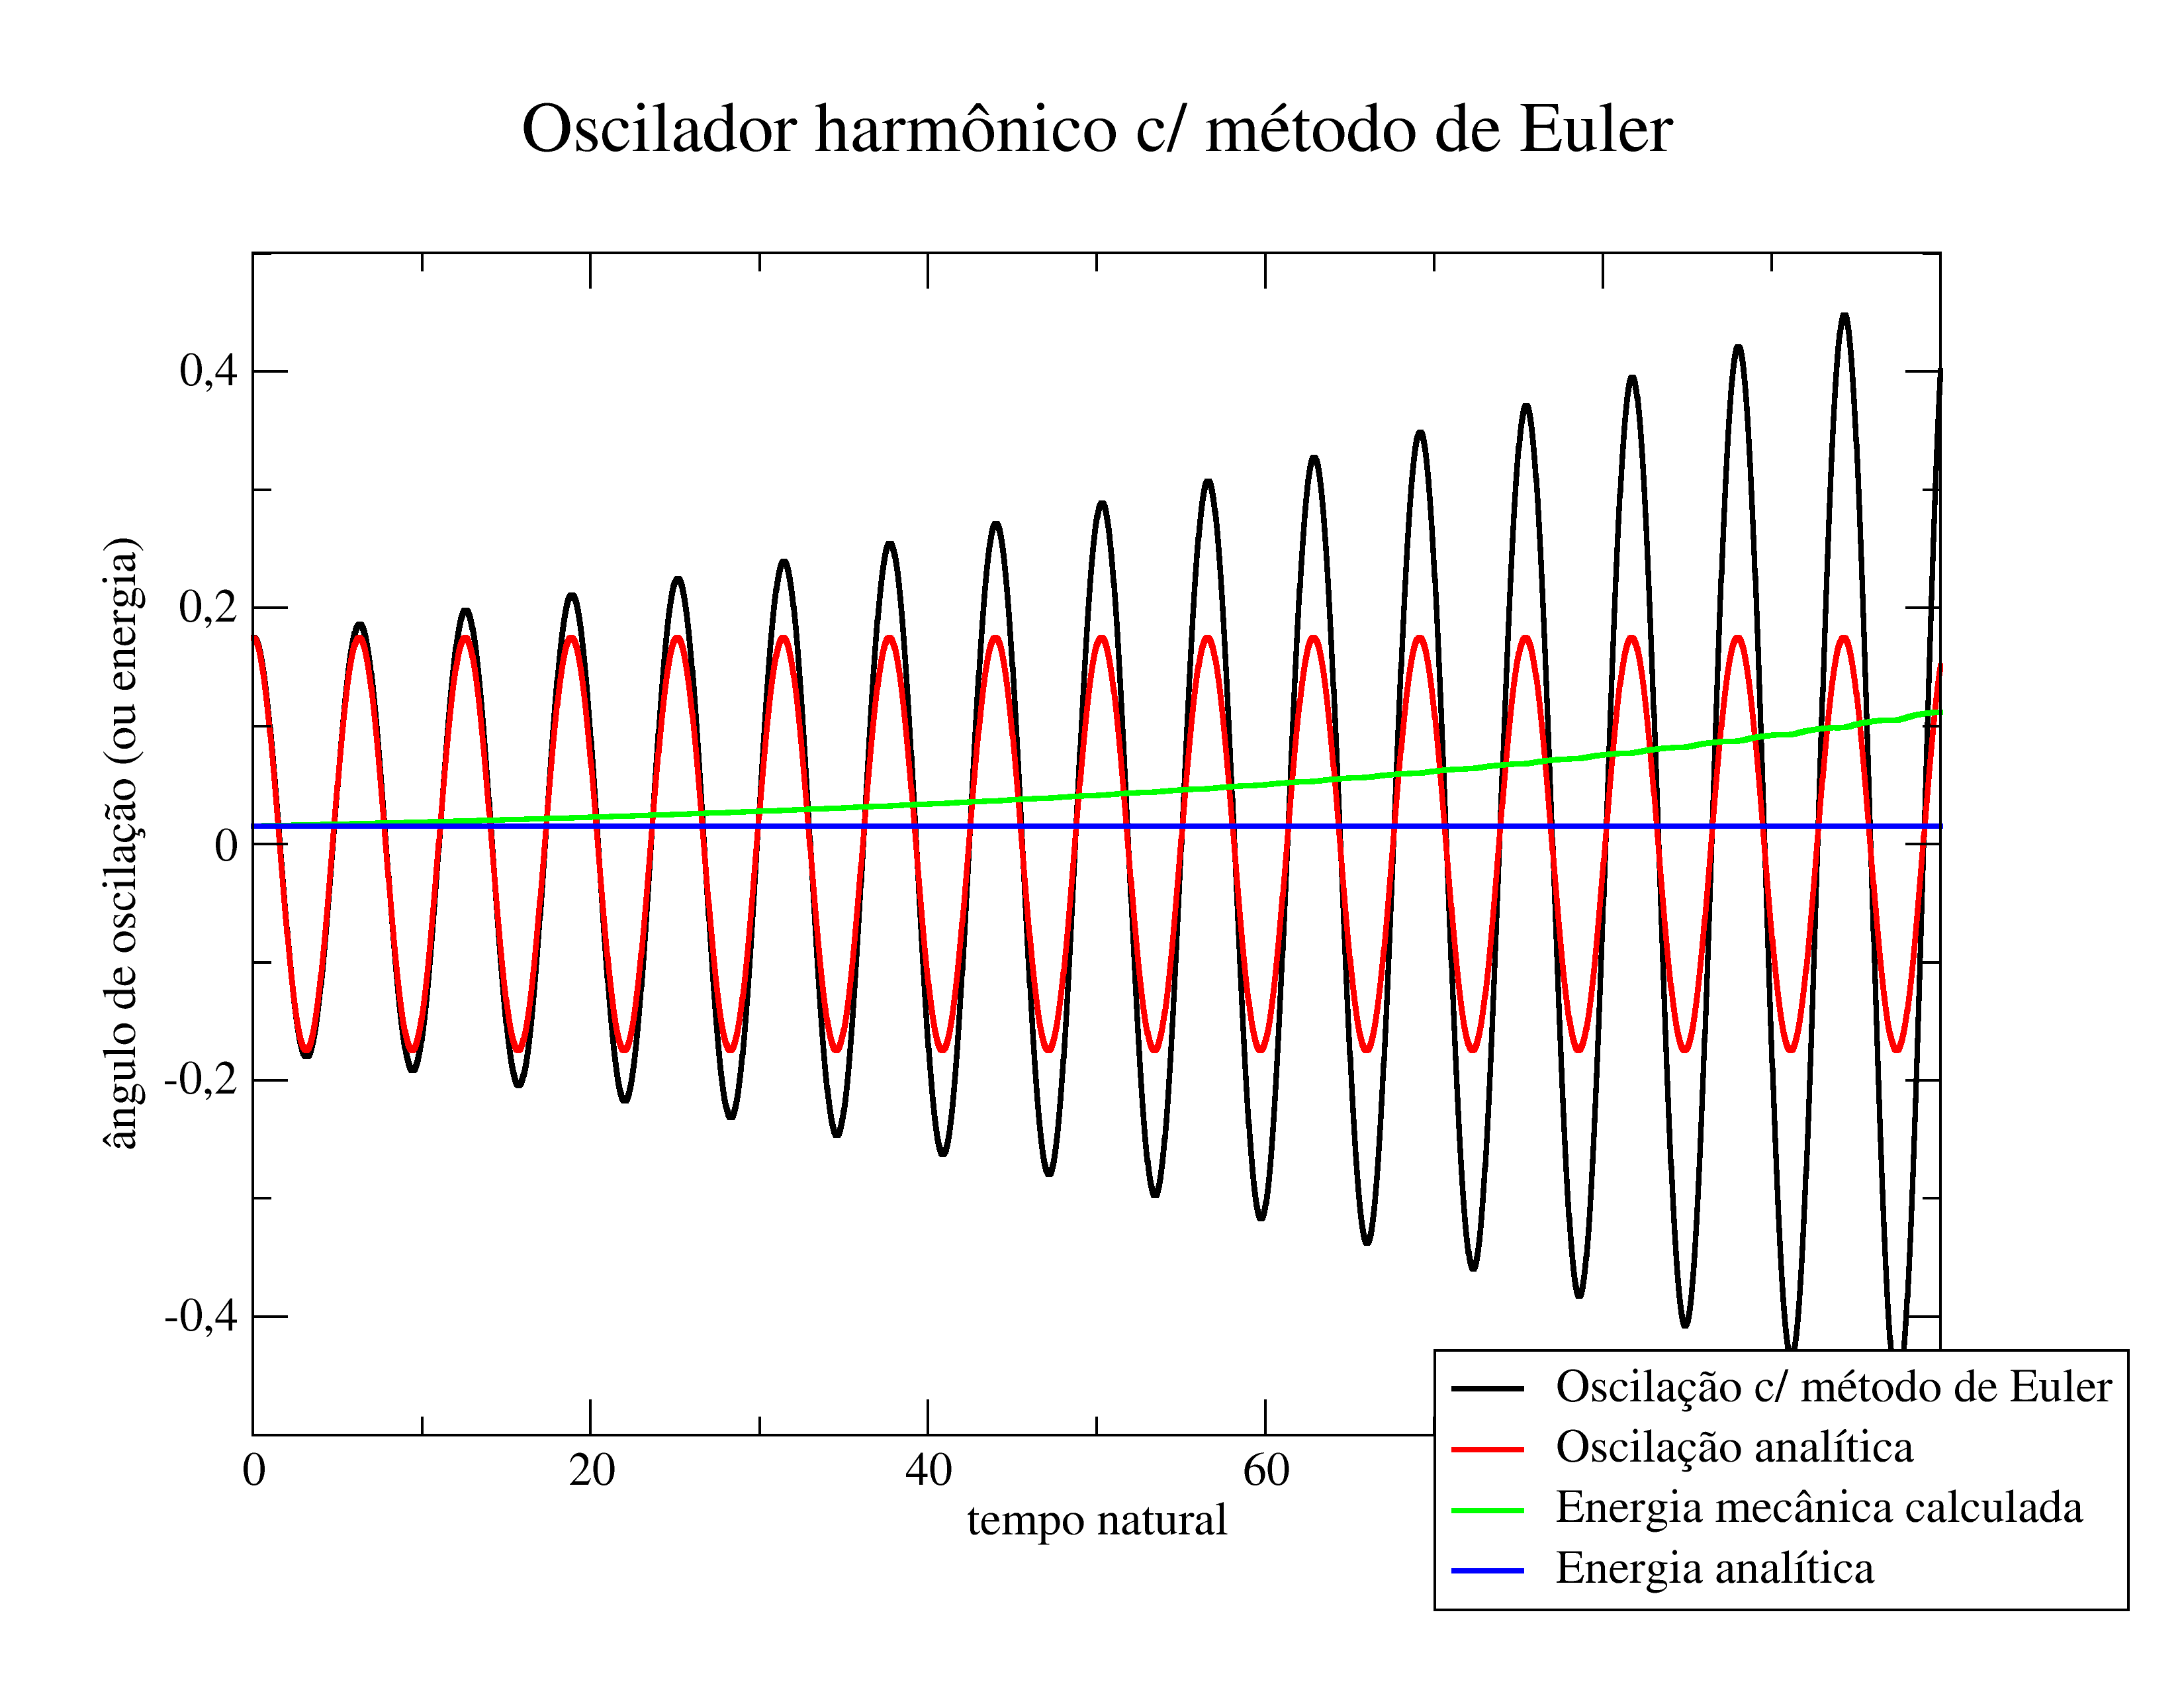
\includegraphics[width=\linewidth]{../tarefa-1a/grafico.png}
\caption{Gráfico do movimento de um oscilador harmônico com o método de Euler e $\theta_0 = 10\degree$.}
\end{figure}

Percebe-se que o movimento, ao longo do tempo, diverge daquilo que é esperado, e o módulo da oscilação vai aumentando ao longo do tempo. Isso também é notado na energia mecânica, que aumenta ao longo do tempo ao invés de permanecer constante. Ou seja, o método de Euler não é adequado para calcular este tipo de movimento ao longo do tempo.

\subsection{b}

Agora apenas substituímos o método de Euler pelo de Euler-Cromer. Segue o programa:

\begin{minted}[
	mathescape,
	linenos,
	fontsize=\footnotesize,
	framesep=2mm,
	breaklines]
	{fortranfixed}
      implicit real*8 (a-h, o-z)

      pi = 4.d0*datan2(1.d0,1.d0)

      w0 = 0d0
      teta0 = pi*10d0/180d0 ! teta0 = 10 graus
      teta0original = teta0
      total_tau = 100
      dtau = 2d-2
      iteracoes = int(total_tau/dtau)

      tetanovo = 0d0
      wnovo = 0d0

      e_mec_anal = 1d0 - dcos(teta0) + 0.5d0*(w0**2d0)

      open(file='tarefa-1-saida.dat', unit=1)
      open(file='saida-analitica.dat', unit=2)
      open(file='energia-harm.dat', unit=3)
      open(file='energia-anal.dat', unit=4)

      do i=1,iteracoes
         tempo = dble(i)*dtau
         write(1,*) tempo, teta0

         wnovo = w0 - teta0*dtau
         tetanovo = teta0 + wnovo*dtau

         ! calcular analitico
         teta_anal = teta0original*dcos(tempo)
         write(2,*) tempo, teta_anal

         ! calcular energia
         e_mec = 1d0 - dcos(teta0) + 0.5d0*(w0**2d0)

         write(3,*) tempo, e_mec
         write(4,*) tempo, e_mec_anal

         w0 = wnovo
         teta0 = tetanovo
      end do


      end

\end{minted}

Graficando isso, temos agora

\begin{figure}[H]
\centering
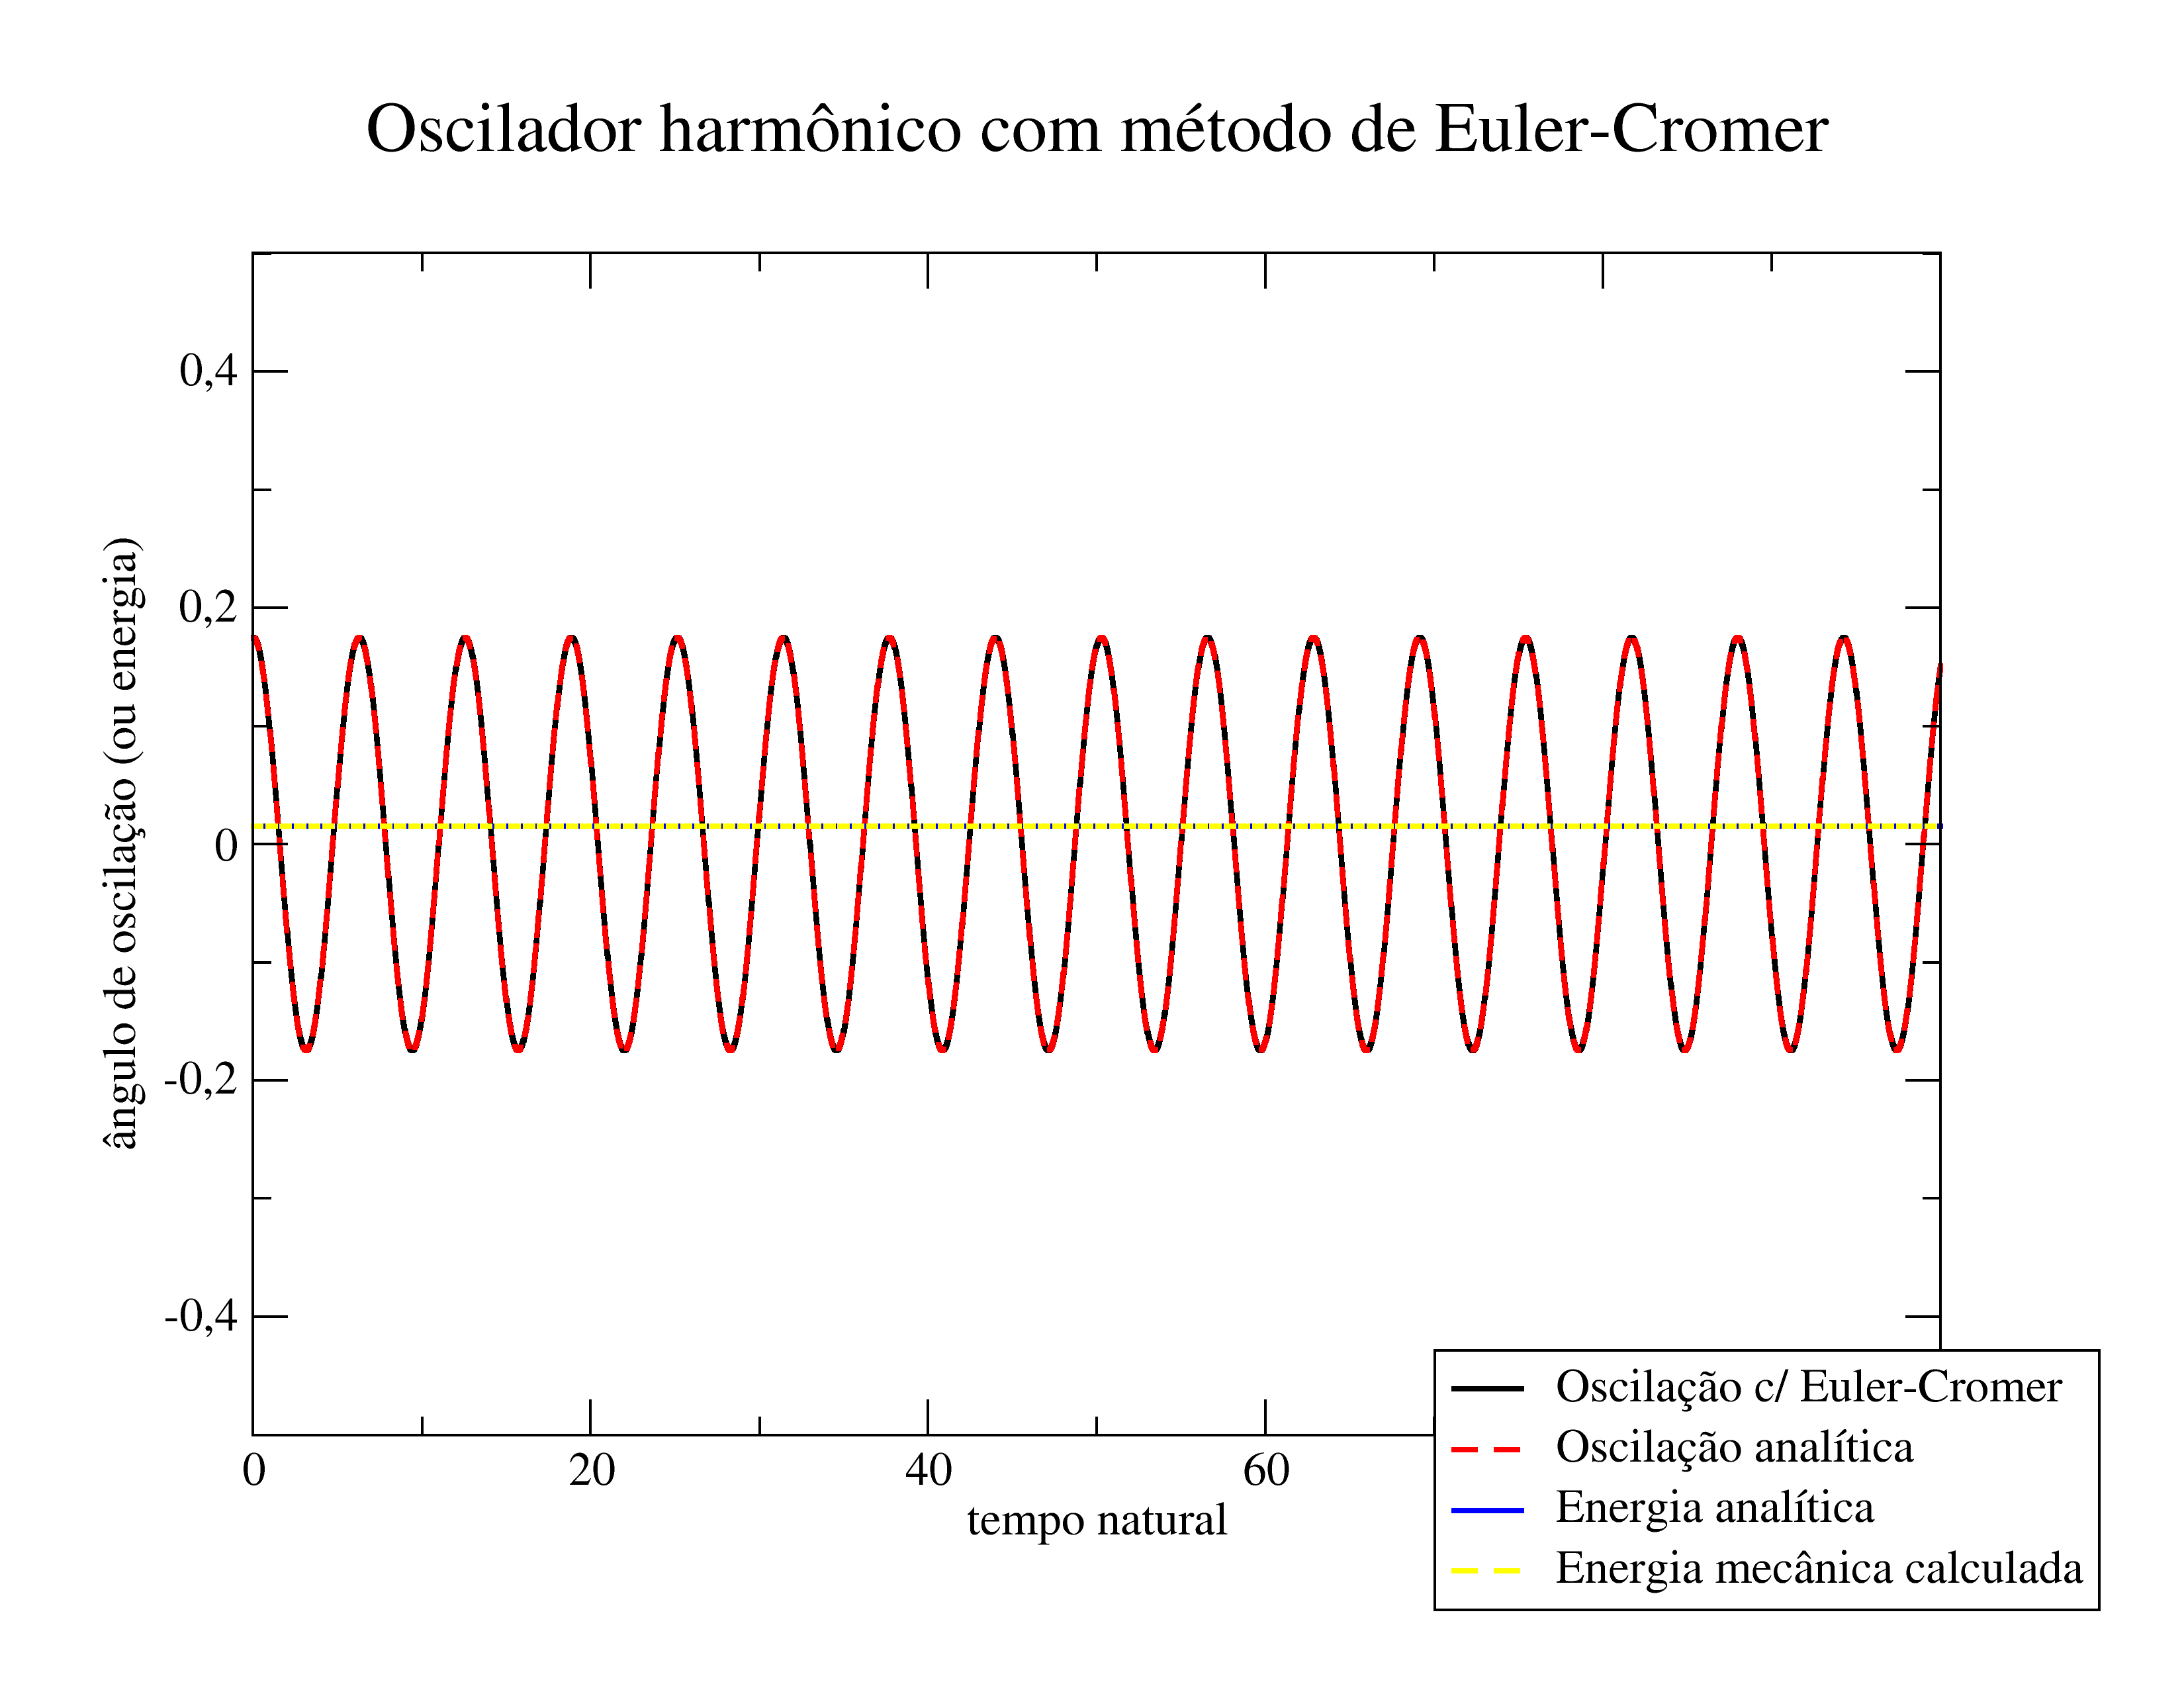
\includegraphics[width=\textwidth]{../tarefa-1b/grafico.png}
\caption{Gráfico do movimento e da energia de um oscilador harmônico via Euler-Cromer.}
\end{figure}

Agora podemos ver que o movimento permanece correto ao longo de toda a simulação, sem divergir, e que a energia mecânica calculada também permanece constante, ou seja, o método de Euler-Cromer parece ser adequado para esse tipo de sistema.

\section{Tarefa 2}
Eu juntei as duas subtarefas (a) e (b) no mesmo programa para facilitar a organização, já que elas são muito parecidas.

Aqui calculamos o período a partir da simulação do pêndulo verificando a diferença de tempo entre as primeiras duas mudanças de sinal no movimento oscilatório. Depois, para calcular o período "analítico" (usando a integral), utilizamos o método de Simpson para cálculo numérico, com $h$ indo de $10^{-9}$ a $10^{-7}$, dependendo da proximidade ao ponto 0 (quanto mais próximo chegamos do 0, maior o erro, portanto precisamos aumentar $h$.) Finalmente, calculamos também a "aproximação" do período dado na tarefa 2-b. Segue o programa:

\begin{minted}[
	mathescape,
	linenos,
	fontsize=\footnotesize,
	framesep=2mm,
	breaklines]
	{fortranfixed}
      implicit real*8 (a-h, o-z)

      pi = 4.d0*datan2(1.d0,1.d0)

      w0 = 0d0

      write(*,*)"Insira o angulo maximo inicial"
      read(*,*)iangulomax

      open(file='tarefa-2-saida.dat', unit=1)
      open(file='periodos-analitico.dat', unit=2)
      open(file='periodo_aprox.dat', unit=3)

      iangulomin = -iangulomax

      total_tau = 100
      dtau = 1d-6
      iteracoes = int(total_tau/dtau)

      tetanovo = 0d0
      wnovo = 0d0

      do iang=iangulomin,iangulomax
         teta0 = pi*dble(iang)/180d0
         teta0original = teta0

         ! Para calcular o período analítico, vamos alterando h conforme chegamos próximo de 0
         ! (isso faz com que tenhamos melhor precisão nos resultados, pois precisamos de subdivisões menores)
         ! E para teta = 0, não teríamos integral nem oscilação, e portanto fazemos simplesmente 2pi, para ter continuidade no gráfico.
         if (abs(iang).lt.10) then
            h = 1d-9
         else if (abs(iang).lt.20) then
            h = 1d-8
         else
            h = 1d-7
         endif
         if (teta0original.eq.0d0) then
            t_anal = 2d0*pi
         else
            t_anal = periodo_anal(teta0original, h)
         endif

         ! Para checar o periodo, vamos calcular quanto tempo passa entre duas mudanças de sinal,
         ! e multiplicar isso por 2

         t_periodo_inicio = 0d0
         t_periodo_fim = 0d0

         do i=1,iteracoes
            tempo = dble(i)*dtau

            wnovo = w0 - dsin(teta0)*dtau
            tetanovo = teta0 + wnovo*dtau

            if ((wnovo*w0).lt.0d0) then
               if (t_periodo_inicio.eq.0d0)then
                  t_periodo_inicio = tempo
               else if (t_periodo_fim.eq.0d0)then
                  t_periodo_fim = tempo
               end if
            end if

            if ((t_periodo_fim*t_periodo_inicio).ne.0d0) then
               goto 10
            end if

            w0 = wnovo
            teta0 = tetanovo
         end do
10       t_periodo = 2d0*(t_periodo_fim - t_periodo_inicio)

         periodo_aprox = 2d0*pi*(1d0 + (1d0/16d0)*(teta0original**2d0))

         write(*,*)"Angulo:",iang,"graus. Periodo calculado:",t_periodo,
     &   "Periodo analitico:", t_anal, "Periodo aprox:", periodo_aprox
         write(1,*)iang,t_periodo
         if (t_anal.gt.0d0) then
            write(2,*)iang,t_anal
         endif
         write(3,*)iang,periodo_aprox

      end do

      end

      function periodo_anal(teta, h)
         implicit real*8 (a-h, o-z)
         real*8 teta, periodo_anal, h, soma, x, simpson, a, b
         ! vamos utilizar a regra de Simpson mas pular a primeira e a última iteração
         ! pois lá teríamos divisão por 0

         teta = dabs(teta)

         a = 0d0
         b = teta

         nparticoes = dint((b-a)/h)

         soma = 0d0

         do i=1,nparticoes-1,2
            x = a + dble(i)*h
            soma = soma + 4.d0/dsqrt(dcos(x)-dcos(teta))
         end do

         do i=2,nparticoes-1,2
            x = a + dble(i)*h
            soma = soma + 2.d0/dsqrt(dcos(x)-dcos(teta))
         end do

         simpson = (h/3.d0) * soma
         simpson = 2d0*dsqrt(2d0)*simpson

         periodo_anal = simpson

      end function

\end{minted}

Graficando os resultados da tarefa 2-a, temos

\begin{figure}[H]
\centering
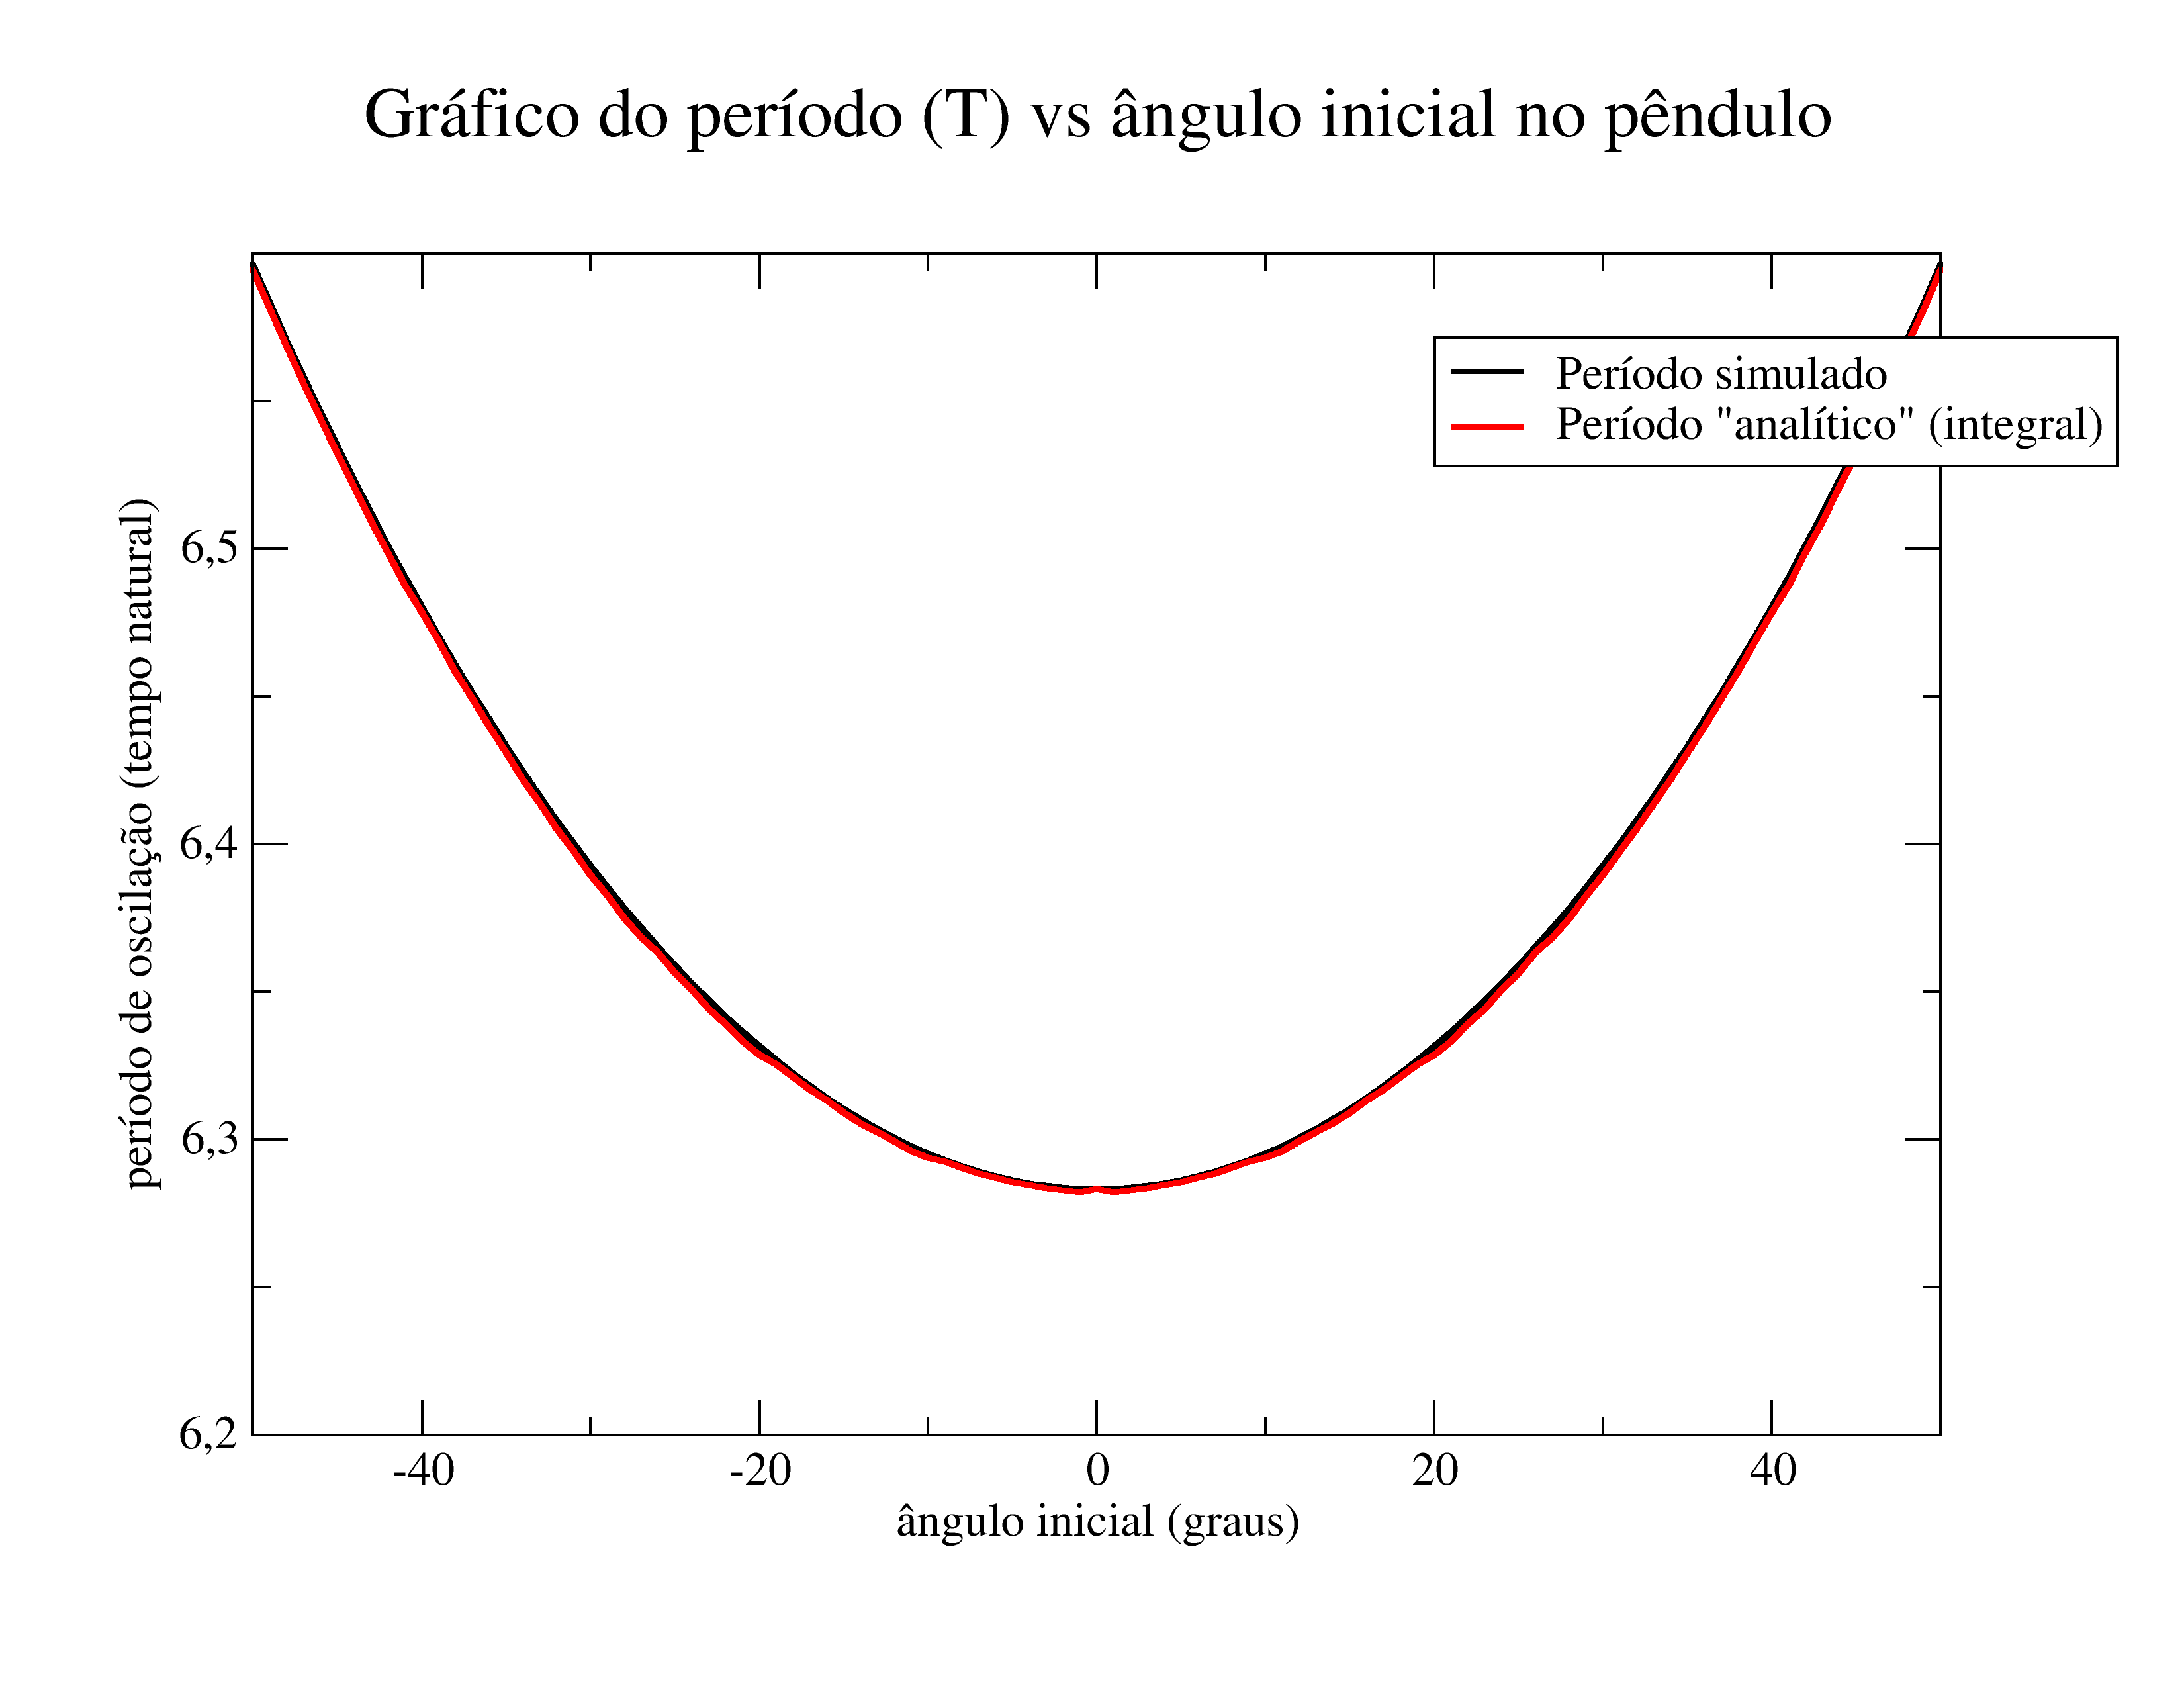
\includegraphics[width=\textwidth]{../tarefa-2a/grafico.png}
\caption{Gráfico do período do oscilador harmônico, com $\theta$ indo até $50\degree$.}
\end{figure}

E da 2-b, temos

\begin{figure}[H]
\centering
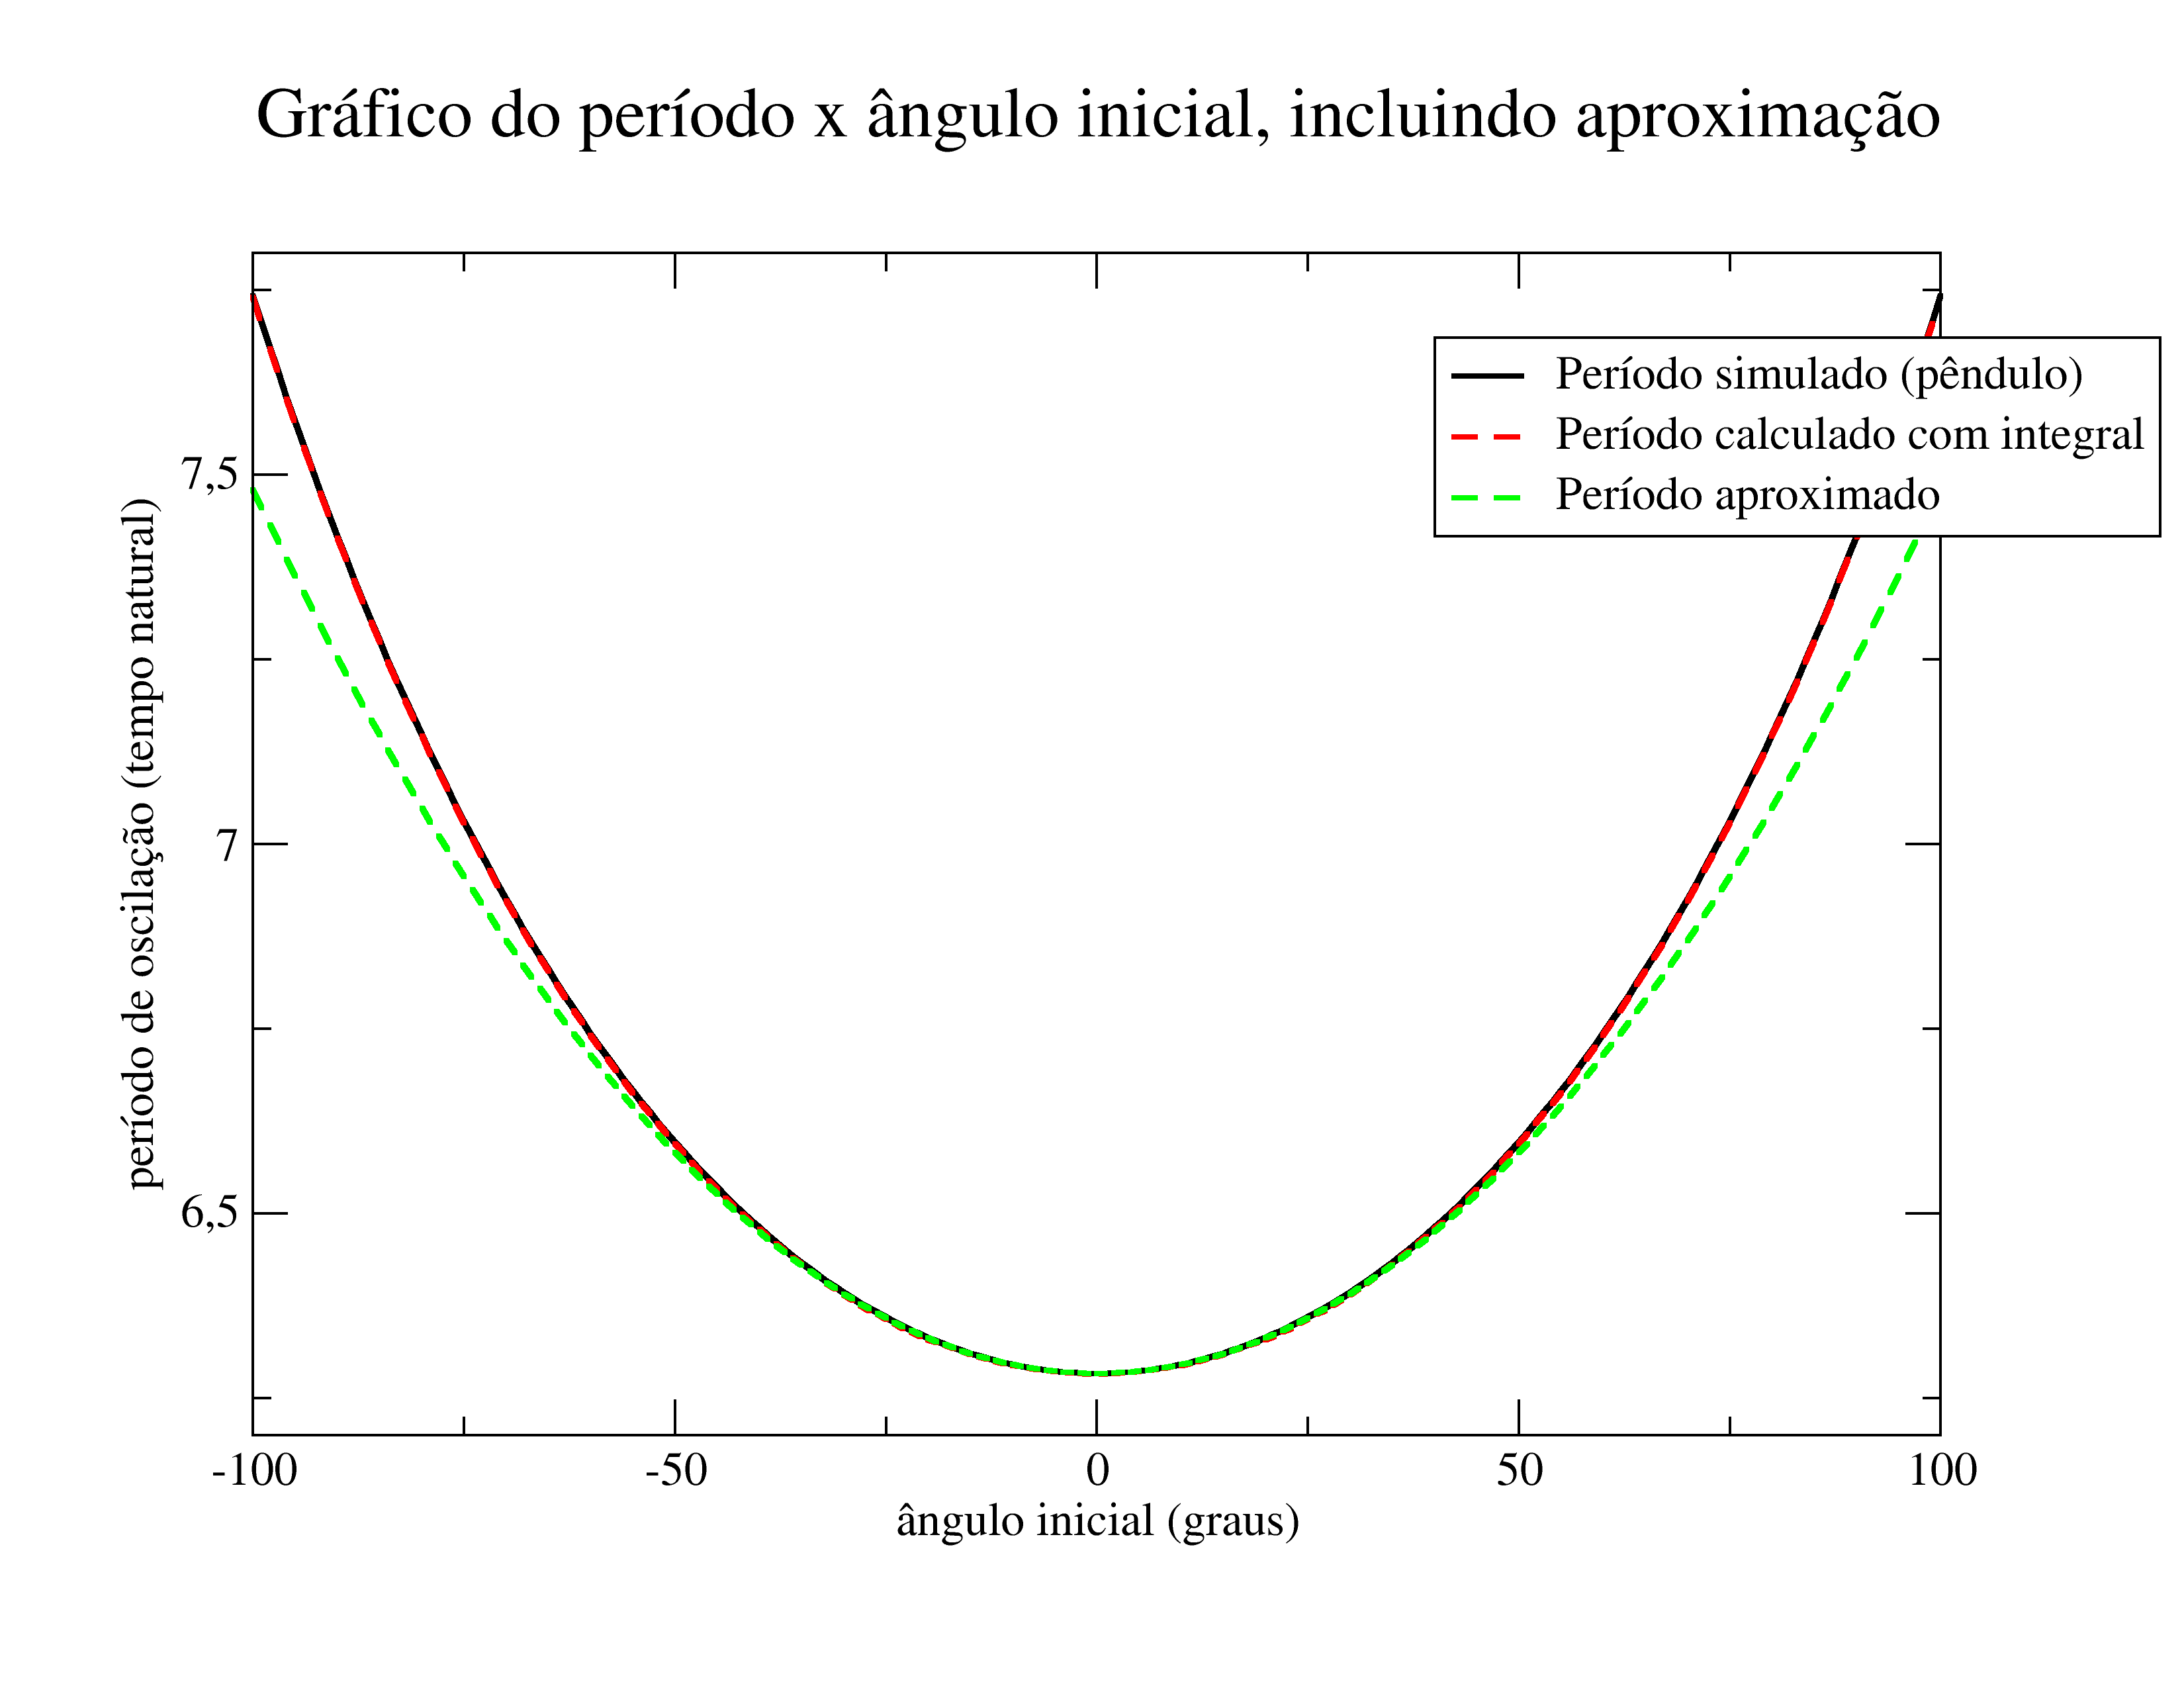
\includegraphics[width=\textwidth]{../tarefa-2a/graficocomaprox.png}
\caption{Gráfico do período do oscilador harmônico, com $\theta$ indo até $100\degree$, incluindo a aproximação polinomial}
\end{figure}

Percebe-se que a aproximação polinomial tem um fitting bem bom da curva real, até cerca de $50\degree$, depois do qual ela passa a divergir cada vez mais da curva correta.

Tabelando os resultados, temos 

\begin{table}[H]
\begin{center}
\begin{tabular}{|c|c|c|c|}
\hline
Theta (graus) & Período Simulado & Período Analítico (integral) & Período Aproximado (polinômio) \\
\hline
0.0 & 6.283186 & 6.283185 & 6.283185 \\
\hline
1.0 & 6.283304 & 6.282030 & 6.283305 \\
\hline
2.0 & 6.283664 & 6.282846 & 6.283664 \\
\hline
3.0 & 6.284262 & 6.283390 & 6.284262 \\
\hline
4.0 & 6.285100 & 6.284636 & 6.285099 \\
\hline
5.0 & 6.286176 & 6.285582 & 6.286176 \\
\hline
6.0 & 6.287494 & 6.286997 & 6.287492 \\
\hline
7.0 & 6.289052 & 6.288463 & 6.289047 \\
\hline
8.0 & 6.290848 & 6.290496 & 6.290841 \\
\hline
9.0 & 6.292888 & 6.292427 & 6.292875 \\
\hline
10.0 & 6.295168 & 6.293890 & 6.295148 \\
\hline
11.0 & 6.297690 & 6.296129 & 6.297660 \\
\hline
12.0 & 6.300454 & 6.299406 & 6.300411 \\
\hline
13.0 & 6.303460 & 6.302498 & 6.303402 \\
\hline
14.0 & 6.306712 & 6.305446 & 6.306631 \\
\hline
15.0 & 6.310208 & 6.309020 & 6.310100 \\
\hline
16.0 & 6.313946 & 6.313244 & 6.313809 \\
\hline
17.0 & 6.317932 & 6.316901 & 6.317756 \\
\hline
18.0 & 6.322164 & 6.321197 & 6.321943 \\
\hline
19.0 & 6.326642 & 6.325442 & 6.326369 \\
\hline
20.0 & 6.331372 & 6.328516 & 6.331034 \\
\hline
21.0 & 6.336350 & 6.333195 & 6.335939 \\
\hline
22.0 & 6.341576 & 6.339084 & 6.341083 \\
\hline
23.0 & 6.347056 & 6.344244 & 6.346466 \\
\hline
24.0 & 6.352790 & 6.350643 & 6.352088 \\
\hline
25.0 & 6.358776 & 6.356286 & 6.357950 \\
\hline
26.0 & 6.365018 & 6.363212 & 6.364050 \\
\hline
27.0 & 6.371516 & 6.368447 & 6.370390 \\
\hline
28.0 & 6.378272 & 6.374985 & 6.376970 \\
\hline
29.0 & 6.385290 & 6.382488 & 6.383788 \\
\hline
30.0 & 6.392568 & 6.389535 & 6.390846 \\
\hline
31.0 & 6.400108 & 6.397563 & 6.398143 \\
\hline
32.0 & 6.407914 & 6.405124 & 6.405679 \\
\hline
33.0 & 6.415986 & 6.413689 & 6.413455 \\
\hline
\end{tabular}
\end{center}
\caption{Tabela para os períodos com $\theta$ indo de $0\degree$ a $33\degree$.}
\end{table}
\newpage

\begin{table}[H]


\begin{center}
\begin{tabular}{|c|c|c|c|}
\hline
Theta (graus) & Período Simulado & Período Analítico (integral) & Período Aproximado (polinômio) \\
\hline
34.0 & 6.424324 & 6.421770 & 6.421469 \\
\hline
35.0 & 6.432936 & 6.430884 & 6.429723 \\
\hline
36.0 & 6.441816 & 6.439492 & 6.438217 \\
\hline
37.0 & 6.450972 & 6.449169 & 6.446949 \\
\hline
38.0 & 6.460404 & 6.458307 & 6.455921 \\
\hline
39.0 & 6.470114 & 6.468565 & 6.465132 \\
\hline
40.0 & 6.480102 & 6.478239 & 6.474582 \\
\hline
41.0 & 6.490376 & 6.487571 & 6.484272 \\
\hline
42.0 & 6.500934 & 6.498523 & 6.494200 \\
\hline
43.0 & 6.511780 & 6.509159 & 6.504368 \\
\hline
44.0 & 6.522916 & 6.520696 & 6.514775 \\
\hline
45.0 & 6.534346 & 6.531904 & 6.525422 \\
\hline
46.0 & 6.546070 & 6.544042 & 6.536308 \\
\hline
47.0 & 6.558094 & 6.555832 & 6.547432 \\
\hline
48.0 & 6.570416 & 6.568584 & 6.558797 \\
\hline
49.0 & 6.583044 & 6.580965 & 6.570400 \\
\hline
50.0 & 6.595982 & 6.594349 & 6.582243 \\
\hline
51.0 & 6.609228 & 6.607332 & 6.594325 \\
\hline
52.0 & 6.622788 & 6.621367 & 6.606646 \\
\hline
53.0 & 6.636666 & 6.634960 & 6.619206 \\
\hline
54.0 & 6.650864 & 6.648316 & 6.632006 \\
\hline
55.0 & 6.665386 & 6.663182 & 6.645045 \\
\hline
56.0 & 6.680238 & 6.677838 & 6.658323 \\
\hline
57.0 & 6.695422 & 6.693375 & 6.671840 \\
\hline
58.0 & 6.710940 & 6.708688 & 6.685597 \\
\hline
59.0 & 6.726798 & 6.724914 & 6.699593 \\
\hline
60.0 & 6.743002 & 6.740900 & 6.713828 \\
\hline
61.0 & 6.759552 & 6.757835 & 6.728302 \\
\hline
62.0 & 6.776458 & 6.774509 & 6.743016 \\
\hline
63.0 & 6.793718 & 6.792176 & 6.757969 \\
\hline
64.0 & 6.811344 & 6.809554 & 6.773161 \\
\hline
65.0 & 6.829336 & 6.827977 & 6.788592 \\
\hline
66.0 & 6.847698 & 6.846075 & 6.804263 \\
\hline
67.0 & 6.866440 & 6.864031 & 6.820173 \\
\hline
\end{tabular}
\end{center}
\caption{Tabela para os períodos com $\theta$ indo de $34\degree$ a $67\degree$.}
\end{table}
\newpage

\begin{table}[H]
\begin{center}
\begin{tabular}{|c|c|c|c|}
\hline
Theta (graus) & Período Simulado & Período Analítico (integral) & Período Aproximado (polinômio) \\
\hline
68.0 & 6.885564 & 6.883469 & 6.836322 \\
\hline
69.0 & 6.905074 & 6.902793 & 6.852710 \\
\hline
70.0 & 6.924980 & 6.923024 & 6.869338 \\
\hline
71.0 & 6.945286 & 6.943132 & 6.886205 \\
\hline
72.0 & 6.965996 & 6.964183 & 6.903311 \\
\hline
73.0 & 6.987120 & 6.985097 & 6.920656 \\
\hline
74.0 & 7.008660 & 7.006995 & 6.938241 \\
\hline
75.0 & 7.030628 & 7.028740 & 6.956065 \\
\hline
76.0 & 7.053024 & 7.051516 & 6.974128 \\
\hline
77.0 & 7.075860 & 7.074116 & 6.992430 \\
\hline
78.0 & 7.099144 & 7.097804 & 7.010972 \\
\hline
79.0 & 7.122880 & 7.121285 & 7.029752 \\
\hline
80.0 & 7.147076 & 7.145921 & 7.048772 \\
\hline
81.0 & 7.171744 & 7.169692 & 7.068032 \\
\hline
82.0 & 7.196886 & 7.194650 & 7.087530 \\
\hline
83.0 & 7.222516 & 7.220589 & 7.107268 \\
\hline
84.0 & 7.248638 & 7.246518 & 7.127245 \\
\hline
85.0 & 7.275268 & 7.273470 & 7.147461 \\
\hline
86.0 & 7.302408 & 7.300405 & 7.167917 \\
\hline
87.0 & 7.330070 & 7.328411 & 7.188612 \\
\hline
88.0 & 7.358268 & 7.356388 & 7.209546 \\
\hline
89.0 & 7.387006 & 7.385492 & 7.230719 \\
\hline
90.0 & 7.416298 & 7.414551 & 7.252131 \\
\hline
91.0 & 7.446156 & 7.444801 & 7.273783 \\
\hline
92.0 & 7.476590 & 7.474983 & 7.295674 \\
\hline
93.0 & 7.507612 & 7.506431 & 7.317804 \\
\hline
94.0 & 7.539236 & 7.537173 & 7.340174 \\
\hline
95.0 & 7.571470 & 7.569221 & 7.362783 \\
\hline
96.0 & 7.604332 & 7.602385 & 7.385631 \\
\hline
97.0 & 7.637834 & 7.635690 & 7.408718 \\
\hline
98.0 & 7.671990 & 7.670164 & 7.432044 \\
\hline
99.0 & 7.706816 & 7.704781 & 7.455610 \\
\hline
100.0 & 7.742324 & 7.740627 & 7.479415 \\
\hline
\end{tabular}
\end{center}
\caption{Tabela para os períodos com $\theta$ indo de $68\degree$ a $100\degree$.}
\end{table}

\section{Tarefa 3}
Aqui o programa é muito parecido com o da tarefa 1-b. Mudamos apenas a expressão para $\ddot{\theta}$, substituindo isso no método de Euler-Cromer. Segue o programa:

\begin{minted}[
	mathescape,
	linenos,
	fontsize=\footnotesize,
	framesep=2mm,
	breaklines]
	{fortranfixed}
      implicit real*8 (a-h, o-z)

      pi = 4.d0*datan2(1.d0,1.d0)

      w0 = 0d0
      teta0 = pi*30d0/180d0
      teta0original = teta0
      total_tau = 40
      dtau = 1d-3
      iteracoes = int(total_tau/dtau)

      gamma = 0.5d0

      tetanovo = 0d0
      wnovo = 0d0

      open(file='tarefa-3-saida.dat', unit=1)

      do i=1,iteracoes
         tempo = dble(i)*dtau
         write(1,*) tempo, teta0

         wnovo = w0 - (dsin(teta0) + gamma*w0)*dtau
         tetanovo = teta0 + wnovo*dtau

         w0 = wnovo
         teta0 = tetanovo
      end do

      end

\end{minted}

Graficando os resultados, temos:

\begin{figure}[H]
\centering
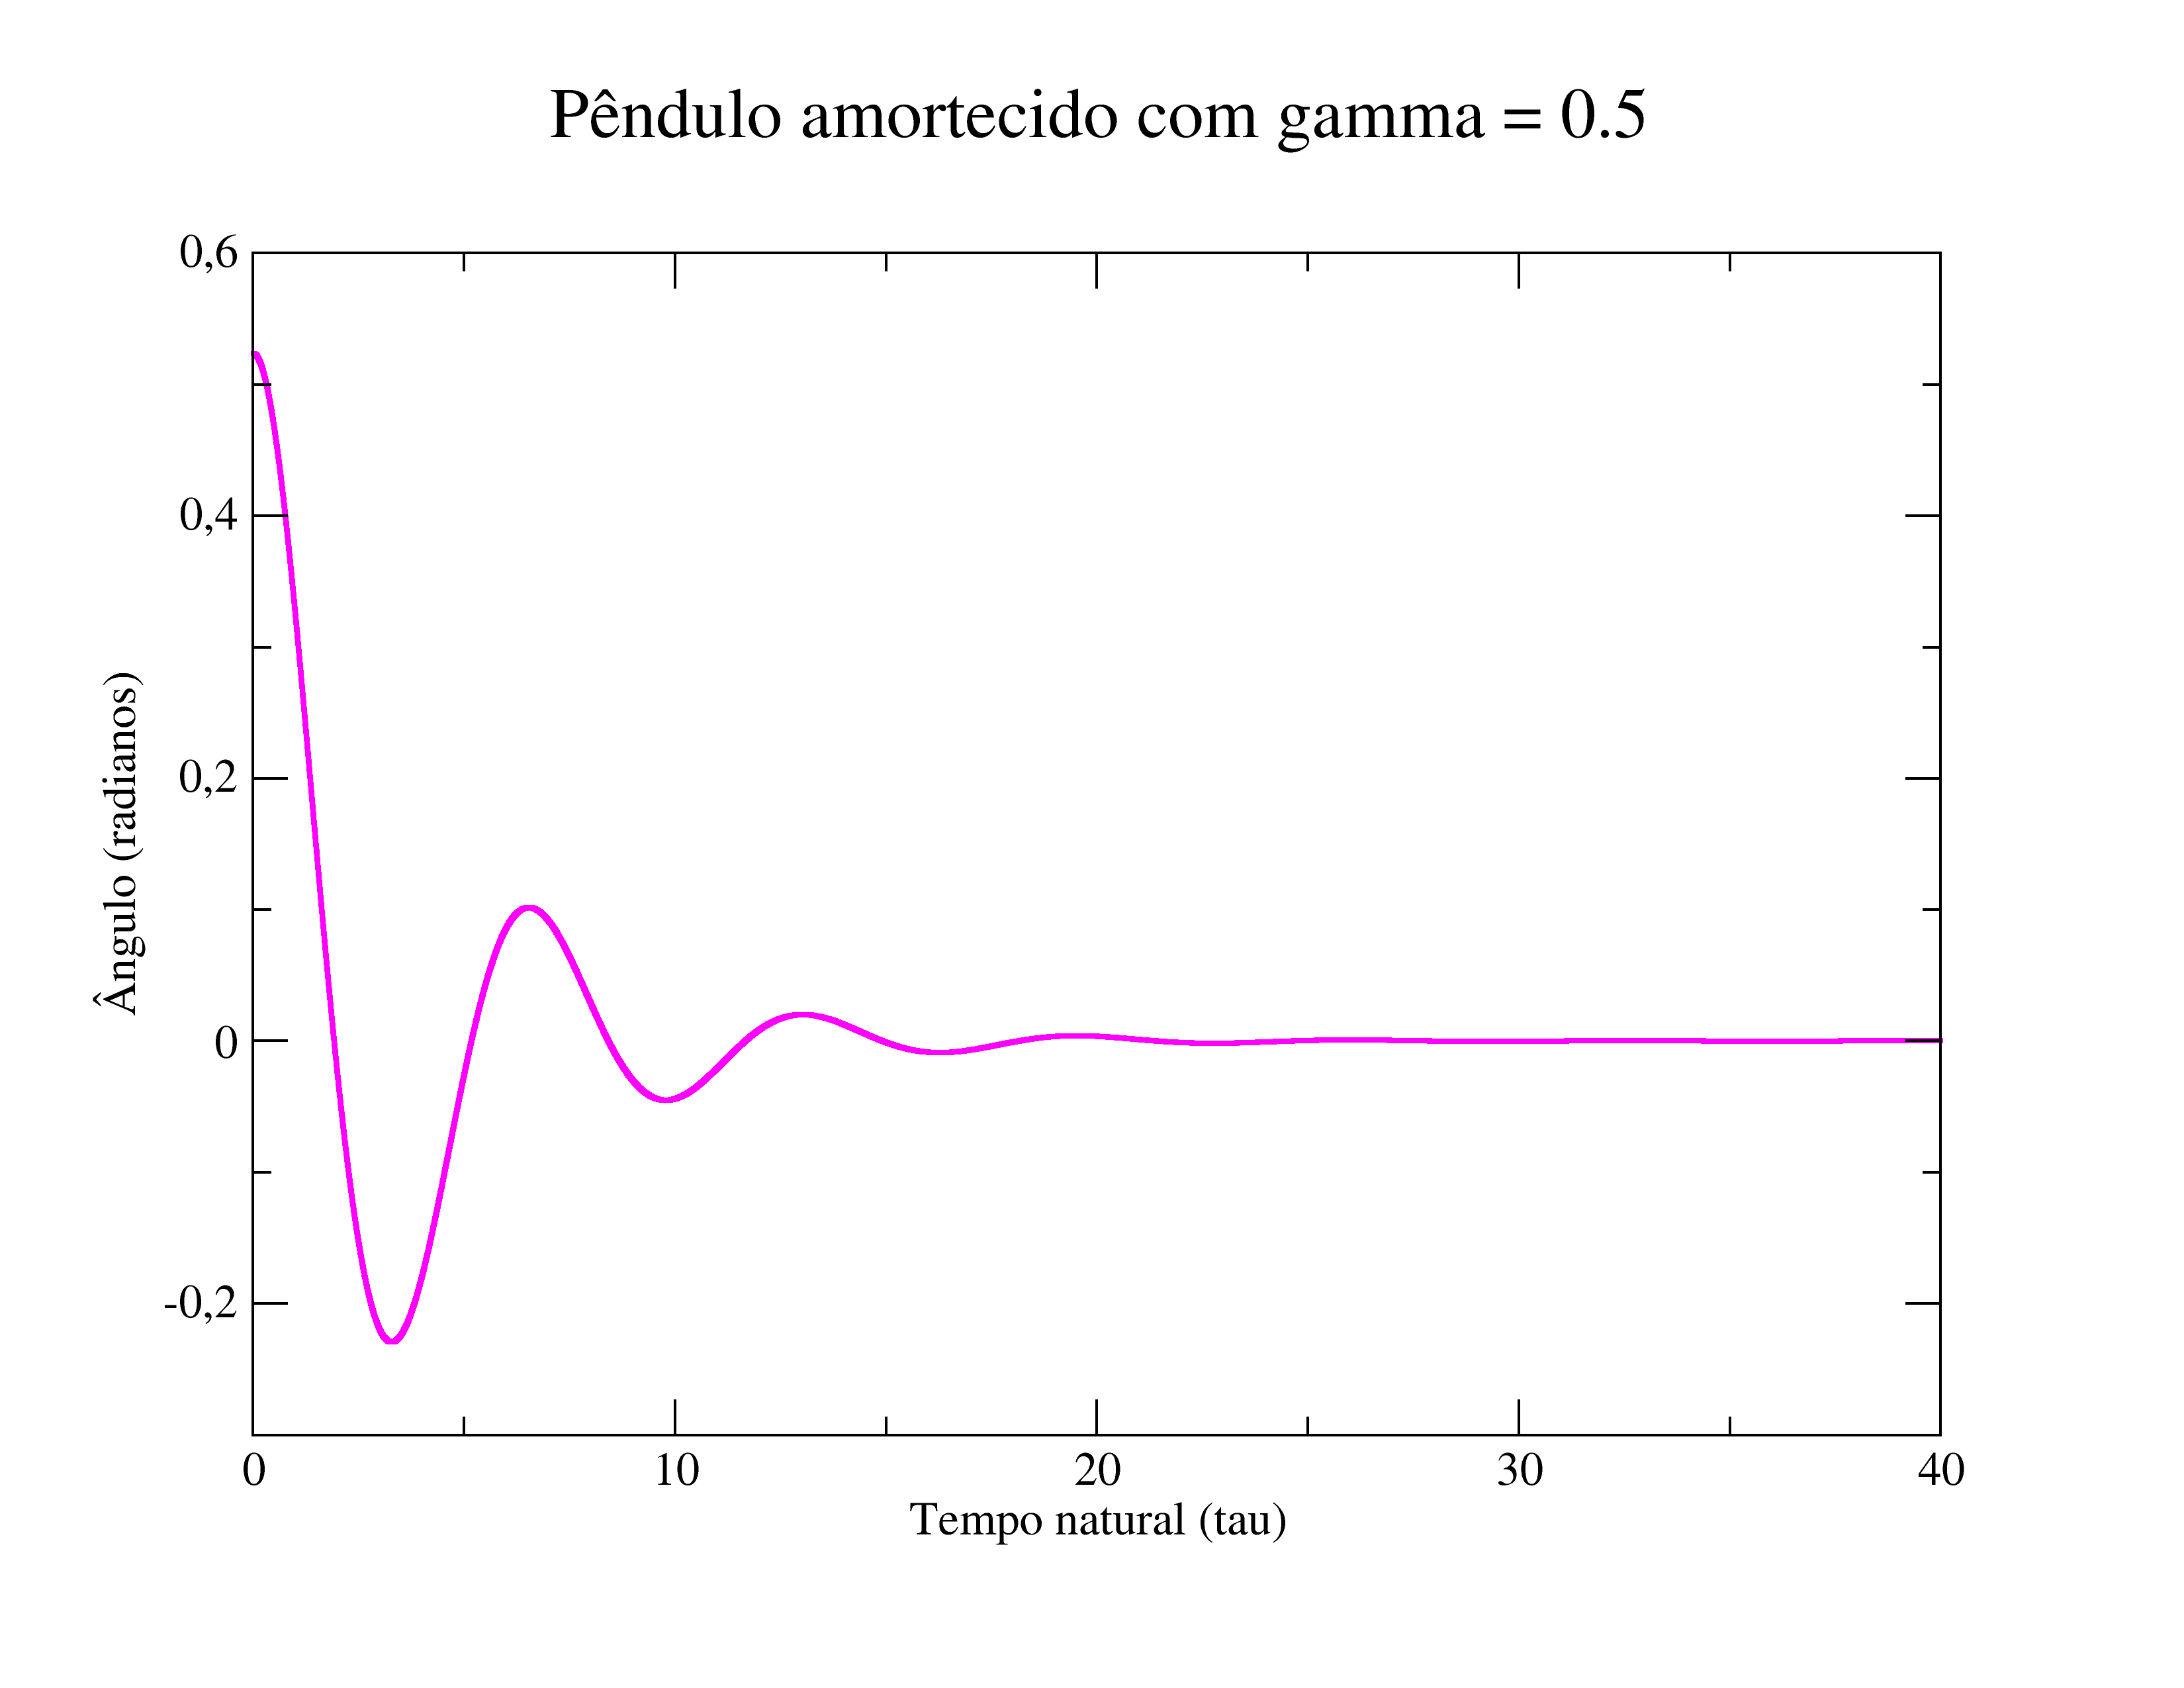
\includegraphics[width=\textwidth]{../tarefa-3/grafico.png}
\caption{Gráfico do pêndulo amortecido.}
\end{figure}

A partir do gráfico, podemos ver que o movimento é de amortecimento sub-crítico, pois há mais do que uma oscilação ao longo do tempo, até que ela finalmente se aquiete após cerca de quatro oscilações.

\section{Tarefa 4}
\subsection{a}
Aqui novamente o programa é muito similar aos anteriores, mudamos apenas a expressão para acomodar a nova força. O programa é:

\begin{minted}[
	mathescape,
	linenos,
	fontsize=\footnotesize,
	framesep=2mm,
	breaklines]
	{fortranfixed}
      implicit real*8 (a-h, o-z)

      pi = 4.d0*datan2(1.d0,1.d0)

      w0 = 0d0
      teta0 = 0d0!pi*30d0/180d0
      teta0original = teta0
      total_tau = 10d0*2d0*pi
      dtau = 1d-3
      iteracoes = int(total_tau/dtau)

      gamma = 0.5d0
      ani = (2d0)/(3d0)

      tetanovo = 0d0
      wnovo = 0d0

      open(file='tarefa-4a-theta.dat', unit=1)
      open(file='tarefa-4a-w.dat', unit=2)
      open(file='tarefa-4a-e.dat', unit=3)

      write(*,*)"Insira alpha"
      read(*,*)alpha

      do i=1,iteracoes
         tempo = dble(i)*dtau

         write(1,*) tempo, teta0
         write(2,*) tempo, w0

         ! calcular energia
         e_mec = 1d0 - dcos(teta0) + 0.5d0*(w0**2d0)

         write(3,*) tempo, e_mec

         !write(*,*)alpha*dsin(ani*tempo), alpha, ani, tempo

         wnovo = w0 -
     &   (dsin(teta0) + gamma*w0 - alpha*dsin(ani*tempo))*dtau

         tetanovo = teta0 + wnovo*dtau

         w0 = wnovo
         teta0 = tetanovo

         teta0 = teta0 - dble(int(teta0/pi))*2d0*pi
      end do

      end

\end{minted}

Graficando todos os resultados, temos

\begin{figure}[H]
\centering
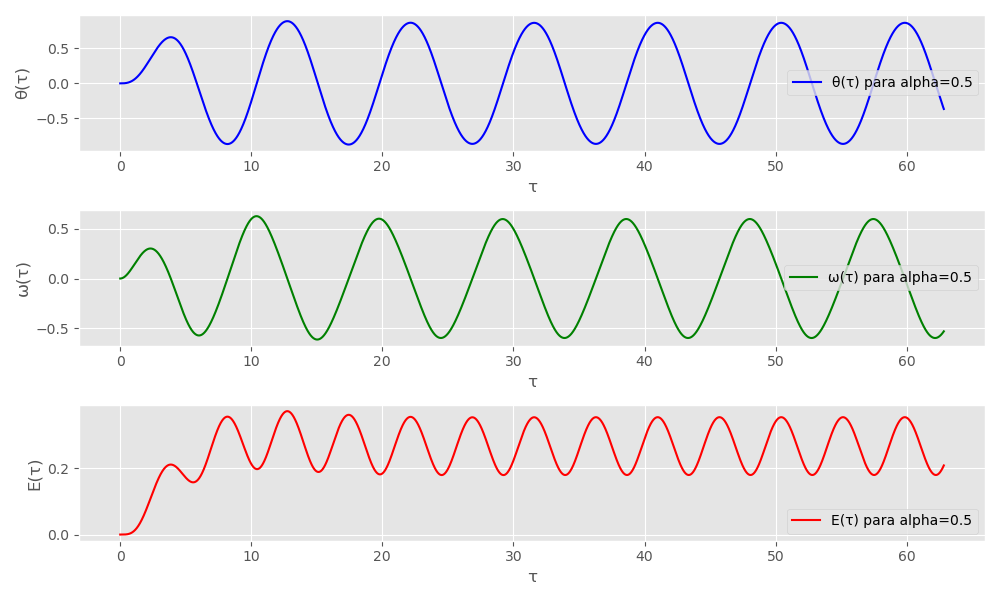
\includegraphics[width=\textwidth]{../tarefa-4a/graficos_alpha_0.5.png}
\caption{Gráfico do pêndulo forçado com $\alpha = 0.5$.}
\end{figure}

\begin{figure}[H]
\centering
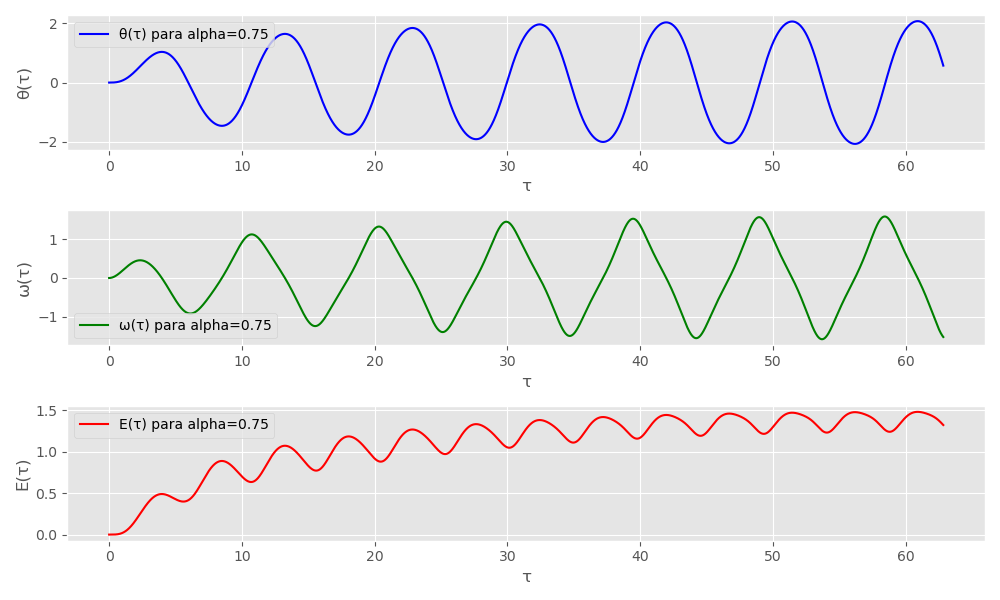
\includegraphics[width=\textwidth]{../tarefa-4a/graficos_alpha_0.75.png}
\caption{Gráfico do pêndulo forçado com $\alpha = 0.75$.}
\end{figure}

\begin{figure}[H]
\centering
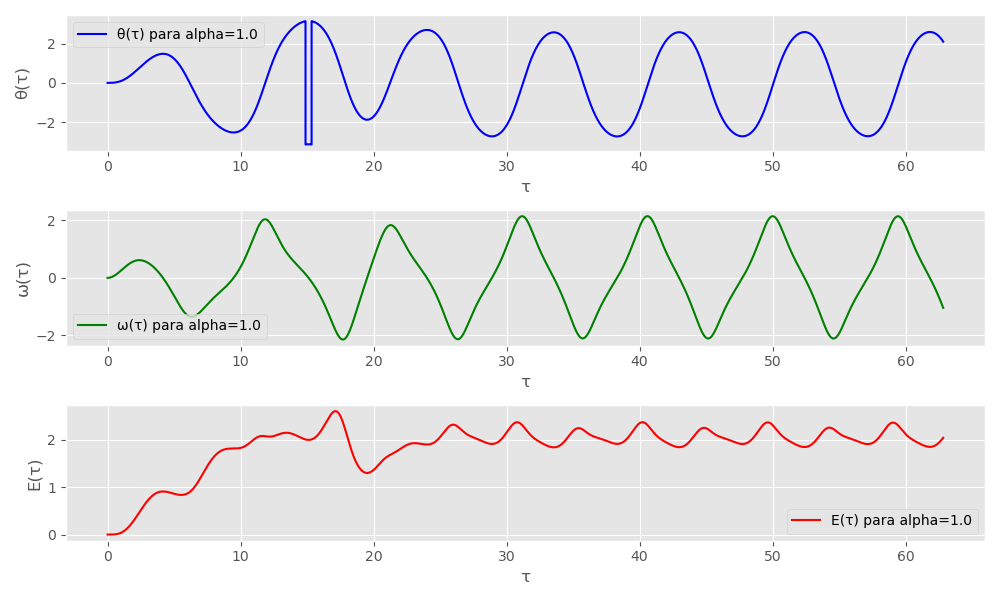
\includegraphics[width=\textwidth]{../tarefa-4a/graficos_alpha_1.0.png}
\caption{Gráfico do pêndulo forçado com $\alpha = 1.0$.}
\end{figure}

\begin{figure}[H]
\centering
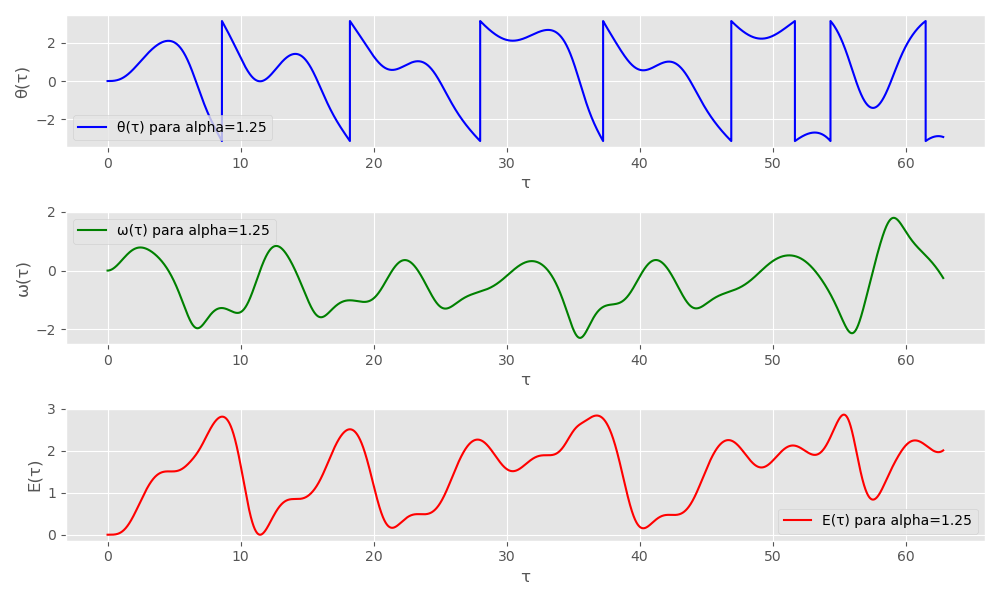
\includegraphics[width=\textwidth]{../tarefa-4a/graficos_alpha_1.25.png}
\caption{Gráfico do pêndulo forçado com $\alpha = 1.25$.}
\end{figure}

\begin{figure}[H]
\centering
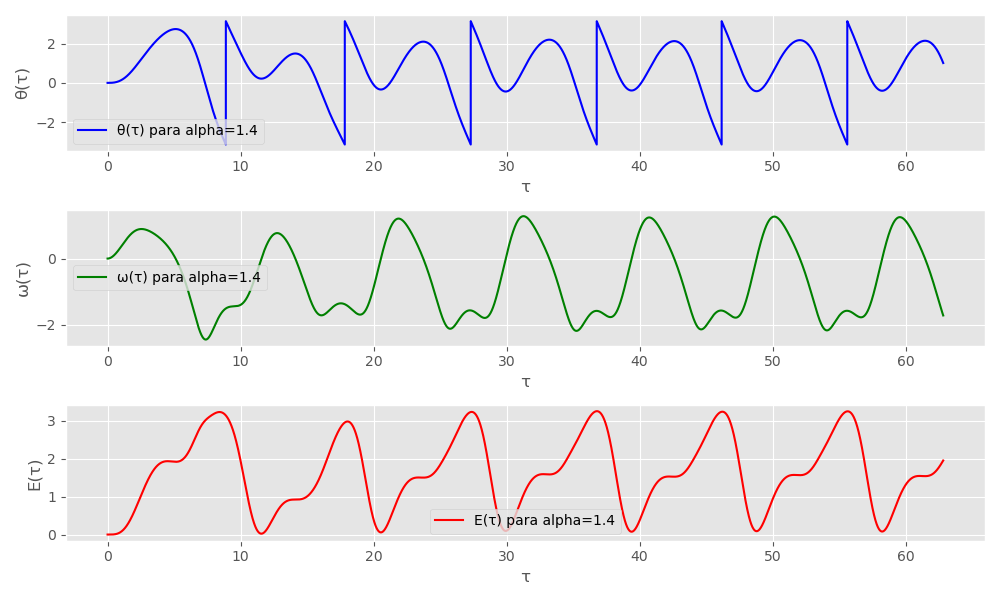
\includegraphics[width=\textwidth]{../tarefa-4a/graficos_alpha_1.4.png}
\caption{Gráfico do pêndulo forçado com $\alpha = 1.4$.}
\end{figure}

\begin{figure}[H]
\centering
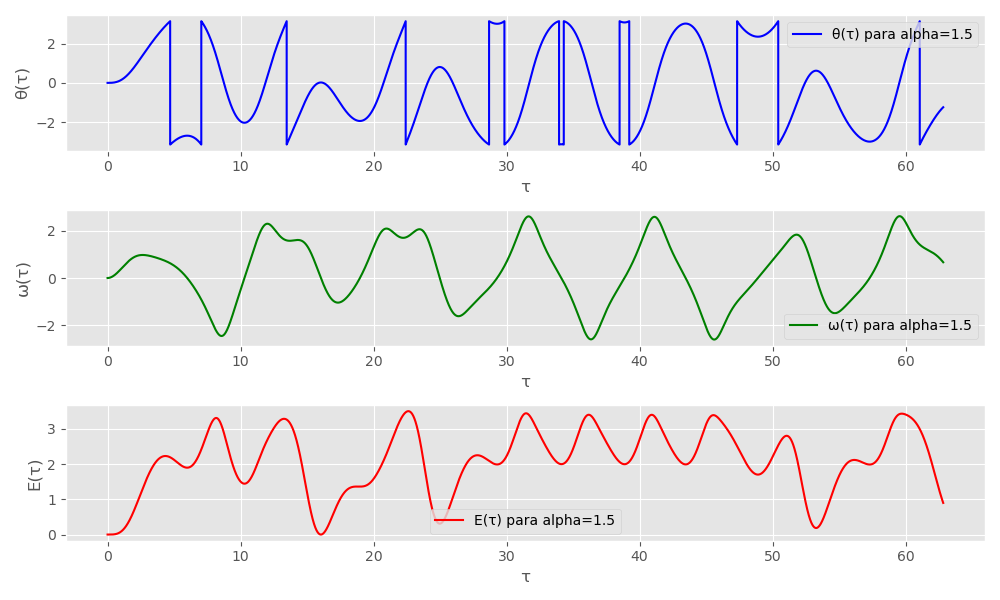
\includegraphics[width=\textwidth]{../tarefa-4a/graficos_alpha_1.5.png}
\caption{Gráfico do pêndulo forçado com $\alpha = 1.5$.}
\end{figure}

Vemos que para $\alpha=0.5,0.75,1.0$ temos um movimento periódico regular. Para $\alpha=1.25,1.5$ temos movimento estritamente não-periódico. E para $\alpha=1.4$, temos movimento "periódico" mas não regular na forma senoidal.

Os tempos $\tau_{trans}$ são aproximadamente $20, 50, 30$ para os três casos periódicos.

\subsection{b}
Agora simplesmente mudamos o programa para graficar $\omega(\theta)$.

\begin{minted}[
	mathescape,
	linenos,
	fontsize=\footnotesize,
	framesep=2mm,
	breaklines]
	{fortranfixed}
      implicit real*8 (a-h, o-z)

      pi = 4.d0*datan2(1.d0,1.d0)

      w0 = 0d0
      teta0 = 0d0!pi*30d0/180d0
      teta0original = teta0
      total_tau = 50d0*2d0*pi
      dtau = 1d-3
      iteracoes = int(total_tau/dtau)

      gamma = 0.5d0
      ani = (2d0)/(3d0)

      tetanovo = 0d0
      wnovo = 0d0

      open(file='tarefa-4b-saida.dat', unit=1)

      write(*,*)"Insira alpha"
      read(*,*)alpha

      do i=1,iteracoes
         tempo = dble(i)*dtau

         write(1,*) teta0, w0

         ! calcular energia
         e_mec = 1d0 - dcos(teta0) + 0.5d0*(w0**2d0)

         !write(*,*)alpha*dsin(ani*tempo), alpha, ani, tempo

         wnovo = w0 -
     &   (dsin(teta0) + gamma*w0 - alpha*dsin(ani*tempo))*dtau

         tetanovo = teta0 + wnovo*dtau

         w0 = wnovo
         teta0 = tetanovo

         teta0 = teta0 - dble(int(teta0/pi))*2d0*pi
      end do

      end

\end{minted}

Graficando os resultados, temos:

\begin{figure}[H]
\centering
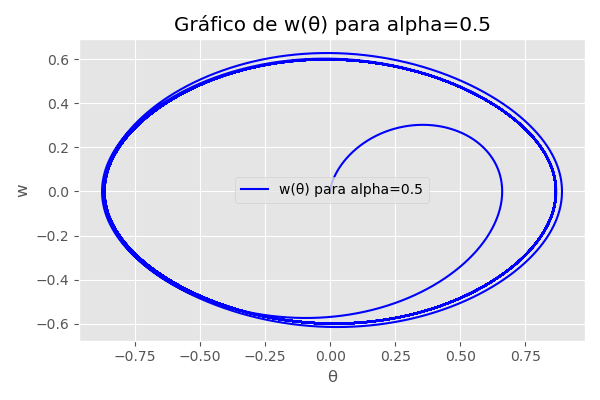
\includegraphics[width=\textwidth]{../tarefa-4b/grafico_w_theta_alpha_0.5.png}
\caption{Gráfico de $\omega(\theta)$ com $\alpha = 0.5$.}
\end{figure}

\begin{figure}[H]
\centering
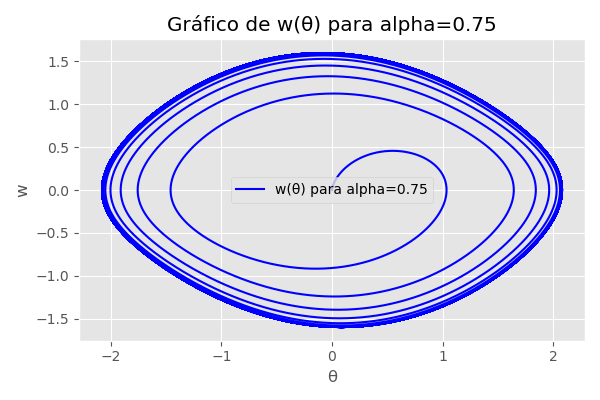
\includegraphics[width=\textwidth]{../tarefa-4b/grafico_w_theta_alpha_0.75.png}
\caption{Gráfico de $\omega(\theta)$ com $\alpha = 0.75$.}
\end{figure}

\begin{figure}[H]
\centering
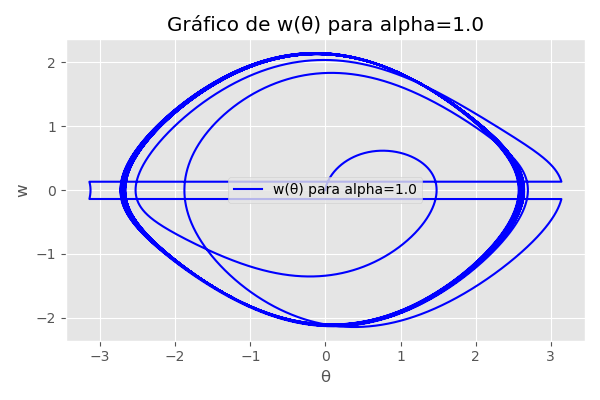
\includegraphics[width=\textwidth]{../tarefa-4b/grafico_w_theta_alpha_1.0.png}
\caption{Gráfico de $\omega(\theta)$ com $\alpha = 1.0$.}
\end{figure}

\begin{figure}[H]
\centering
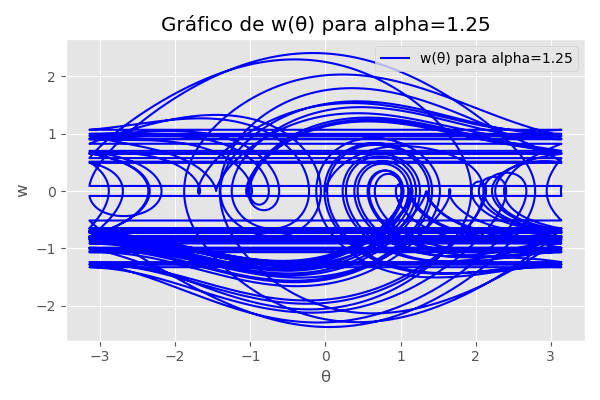
\includegraphics[width=\textwidth]{../tarefa-4b/grafico_w_theta_alpha_1.25.png}
\caption{Gráfico de $\omega(\theta)$ com $\alpha = 1.25$.}
\end{figure}

\begin{figure}[H]
\centering
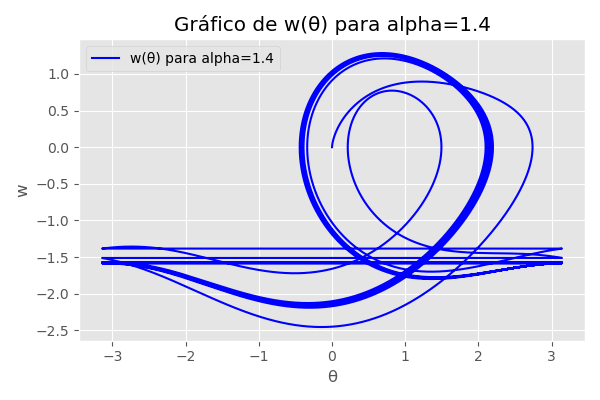
\includegraphics[width=\textwidth]{../tarefa-4b/grafico_w_theta_alpha_1.4.png}
\caption{Gráfico de $\omega(\theta)$ com $\alpha = 1.4$.}
\end{figure}

\begin{figure}[H]
\centering
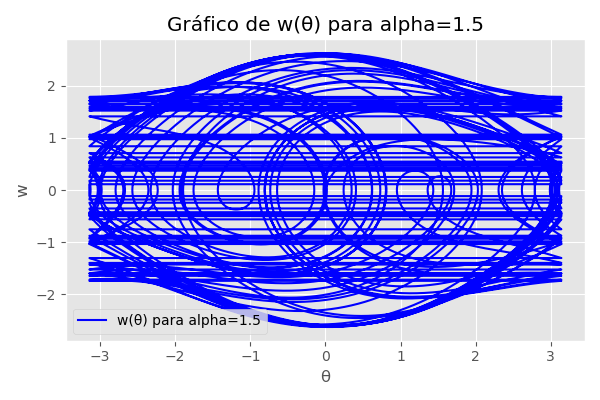
\includegraphics[width=\textwidth]{../tarefa-4b/grafico_w_theta_alpha_1.5.png}
\caption{Gráfico de $\omega(\theta)$ com $\alpha = 1.5$.}
\end{figure}

Vemos que, para os primeiros três casos, temos a emergência de um "círculo-limite", o que faz sentido devido à sua periodicidade. Enquanto que nos outros casos, o gráfico é bem caótico.

\subsection{c}
Aqui, fazemos um programa muito parecido ao anterior, mas dessa vez pegamos como input também o $\tau_{trans}$. Variamos o $\theta_0$ e $\omega_0$, graficando a sobreposição de todos os valores. Segue o programa:

\begin{minted}[
	mathescape,
	linenos,
	fontsize=\footnotesize,
	framesep=2mm,
	breaklines]
	{fortranfixed}
      implicit real*8 (a-h, o-z)
      implicit integer*16 (i-n)

      pi = 4.d0*datan2(1.d0,1.d0)

      w0 = 0d0
      teta0 = 0d0
      teta0original = teta0
      total_tau = 1000d0*2d0*pi
      !total_tau = 1d4*2d0*pi
      dtau = 1d-3
      iteracoes = dint(total_tau/dtau)
      gamma = 0.15d0
      ani = (2d0)/(3d0)

      tetanovo = 0d0
      wnovo = 0d0

      open(file='tarefa-4b-saida.dat', unit=1)

      write(*,*)"Insira alpha"
      read(*,*)alpha

      write(*,*)"Insira t_trans"
      read(*,*)t_trans

      write(*,*)"Insira teta0"
      read(*,*)teta0
      write(*,*)"Insira w0"
      read(*,*)w0

      text = 2d0*pi/ani

      do i=1,iteracoes
         tempo = dble(i)*dtau

         !write(1,*)tempo, text, mod(tempo,text)

         if ((( mod(tempo,text)).lt.1d-3).and.(tempo.gt.t_trans))then
            write(1,*) teta0, w0
         endif

         wnovo = w0 -
     &   (dsin(teta0) + gamma*w0 - alpha*dsin(ani*tempo))*dtau

         tetanovo = teta0 + wnovo*dtau

         w0 = wnovo
         teta0 = tetanovo

         teta0 = teta0 - dble(int(teta0/pi))*2d0*pi
      end do

      end

\end{minted}

Foi utilizado o seguinte programa em Python para gerar os gráficos:

\begin{minted}[
	mathescape,
	linenos,
	fontsize=\footnotesize,
	framesep=2mm,
	breaklines]
	{python}
import subprocess
import matplotlib.pyplot as plt
import numpy as np
import itertools

# Configurar para tema escuro
plt.style.use('dark_background')

# Alphas e t_trans
#alphas = [0.5, 0.75, 1.0, 1.25, 1.4, 1.5, 1.2, 10.0]
#t_trans = [20.0, 50.0, 30.0, 0.0, 0.0, 0.0, 0.0, 0.0]
alphas = [1.2]
t_trans = [0.0]

# Valores iniciais de teta0 e w0
teta0_values = [0, 0.01 * np.pi, 0.02 * np.pi, 0.03 * np.pi]
w0_values = [0, 1e-3, 1e-4, 5e-4, 5e-3, 1e-4]
#teta0_values = [0, 0.5*np.pi]#, 1*np.pi]
#teta0_values=[0]
#w0_values = [1, 1e-3, 1e-4, 1e-1]

# Paleta de cores neon
colors = ['magenta', 'lime', 'cyan', 'yellow', 'orange', 'hotpink', 'red', 'violet', 'aqua', 'orangered', 'crimson']

# Compilar o código Fortran
subprocess.run(["gfortran", "-o", "tarefa-4c.exe", "tarefa-4c.f"])

for i, (alpha, trans) in enumerate(zip(alphas, t_trans)):
    print("plotando i", str(i), alpha)

    plt.figure(figsize=(12, 8))

    for (teta0, w0), color in zip(itertools.product(teta0_values, w0_values), itertools.cycle(colors)):
        # Executar o programa Fortran com os valores atuais
        input_values = f"{alpha:.8f}d0\n{trans:.8f}d0\n{teta0:.8f}d0\n{w0:.8f}d0\n"
        subprocess.run(["./tarefa-4c.exe"], input=input_values.encode())

        # Ler os dados do arquivo
        theta, w = np.loadtxt('tarefa-4b-saida.dat', unpack=True)

        # Tamanho dos símbolos
        marker_size = 1 #if i < 3 else 1

        # Plotar os dados
        plt.plot(theta, w, 'o', color=color, markersize=marker_size)

    # Ajustar os limites dos eixos para os primeiros três alphas
    if i < 3:
        plt.xlim(-np.pi, np.pi)
        plt.ylim(-1, 1)

    plt.xlabel('θ')
    plt.ylabel('w')
    plt.title(f'Seção de Poincaré para alpha={alpha}')
    plt.tight_layout()
    plt.savefig(f'secao_poincare_alpha_{alpha}.png')
    plt.close()

\end{minted}

Executando tudo isso e graficando, temos:

\begin{figure}[H]
\centering
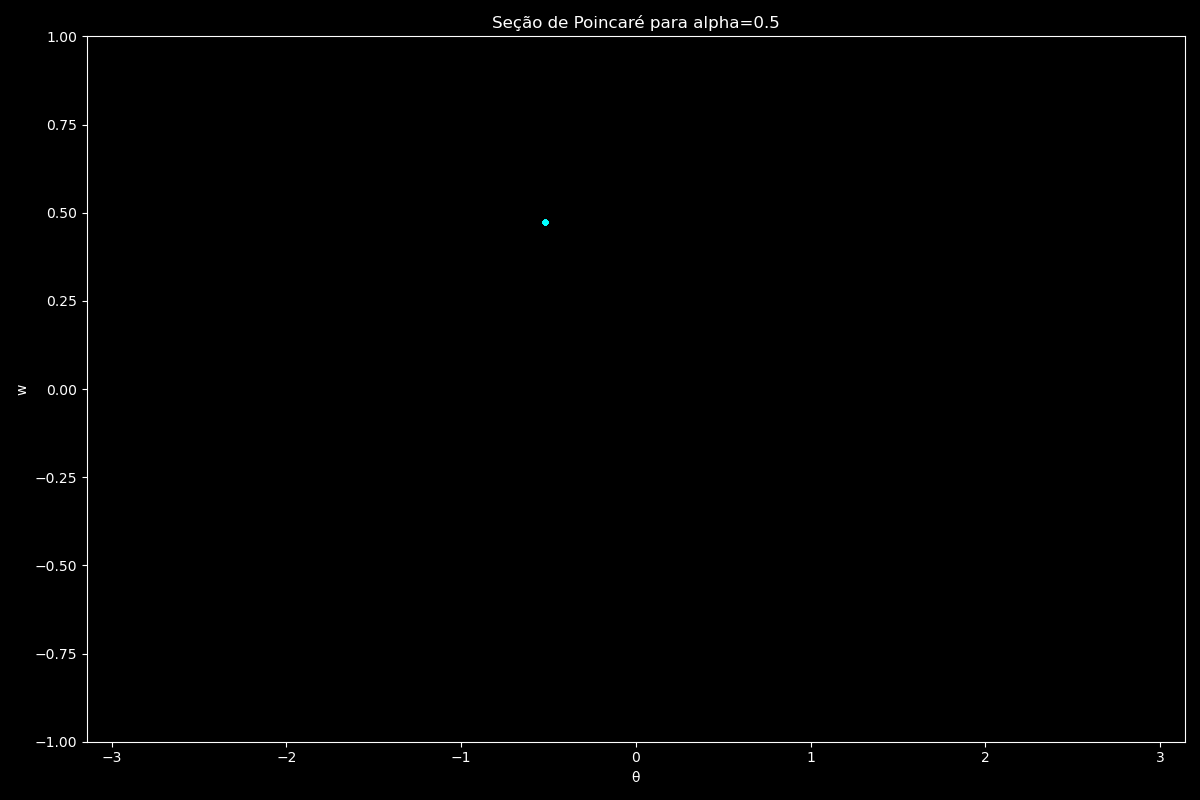
\includegraphics[width=\textwidth]{../tarefa-4c/secao_poincare_alpha_0.5.png}
\caption{Seção de poincaré para $\alpha = 0.5$.}
\end{figure}

\begin{figure}[H]
\centering
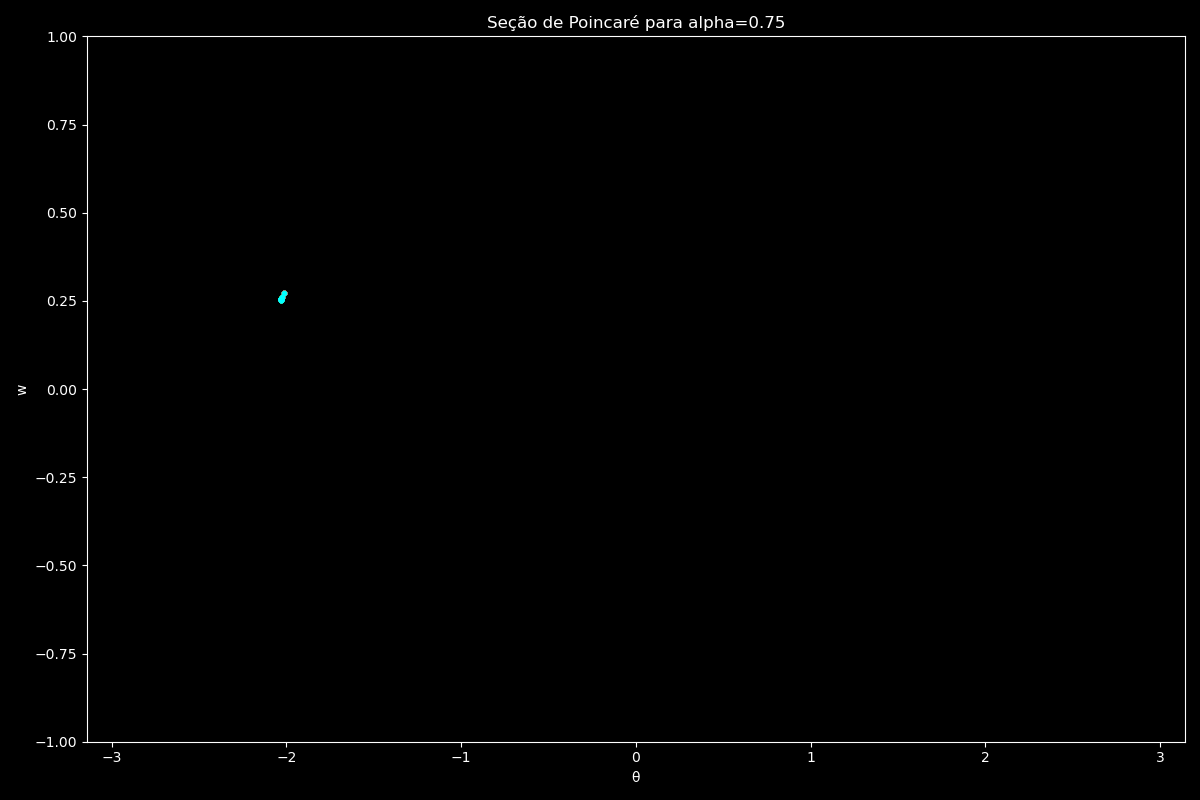
\includegraphics[width=\textwidth]{../tarefa-4c/secao_poincare_alpha_0.75.png}
\caption{Seção de poincaré para $\alpha = 0.75$.}
\end{figure}

\begin{figure}[H]
\centering
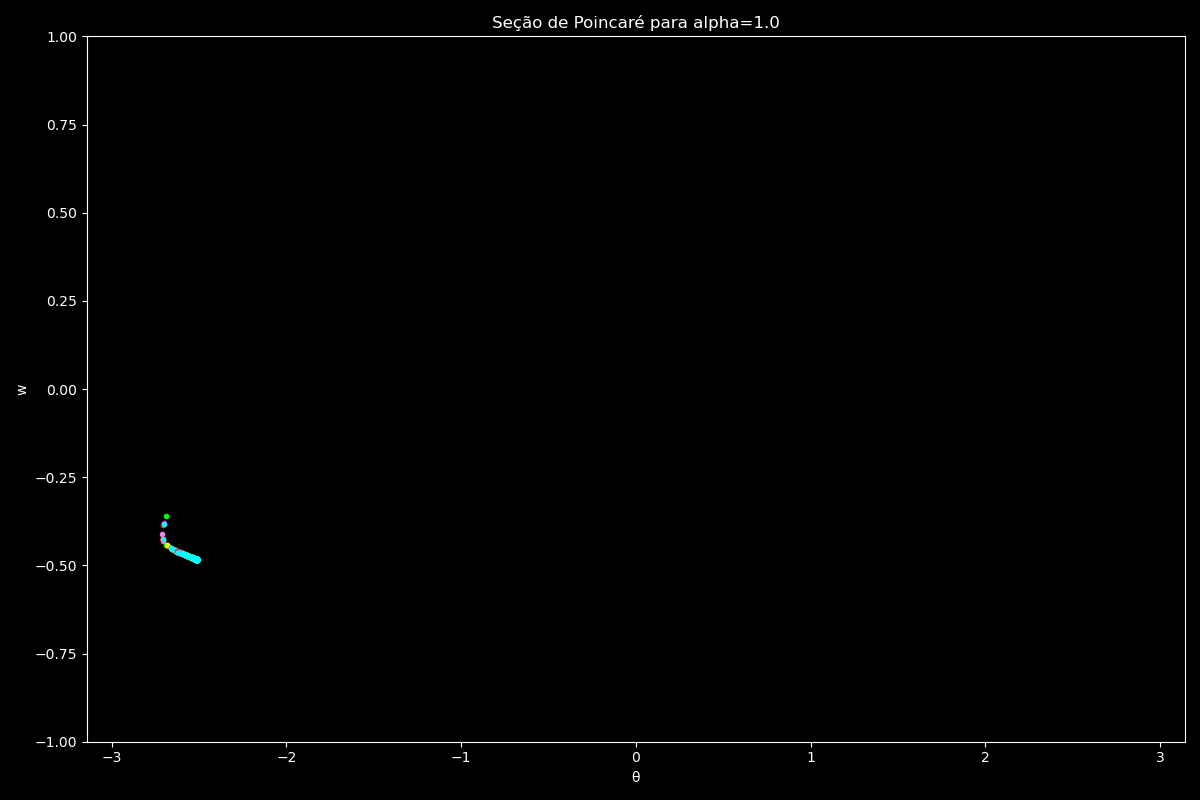
\includegraphics[width=\textwidth]{../tarefa-4c/secao_poincare_alpha_1.0.png}
\caption{Seção de poincaré para $\alpha = 1.0$.}
\end{figure}

\begin{figure}[H]
\centering
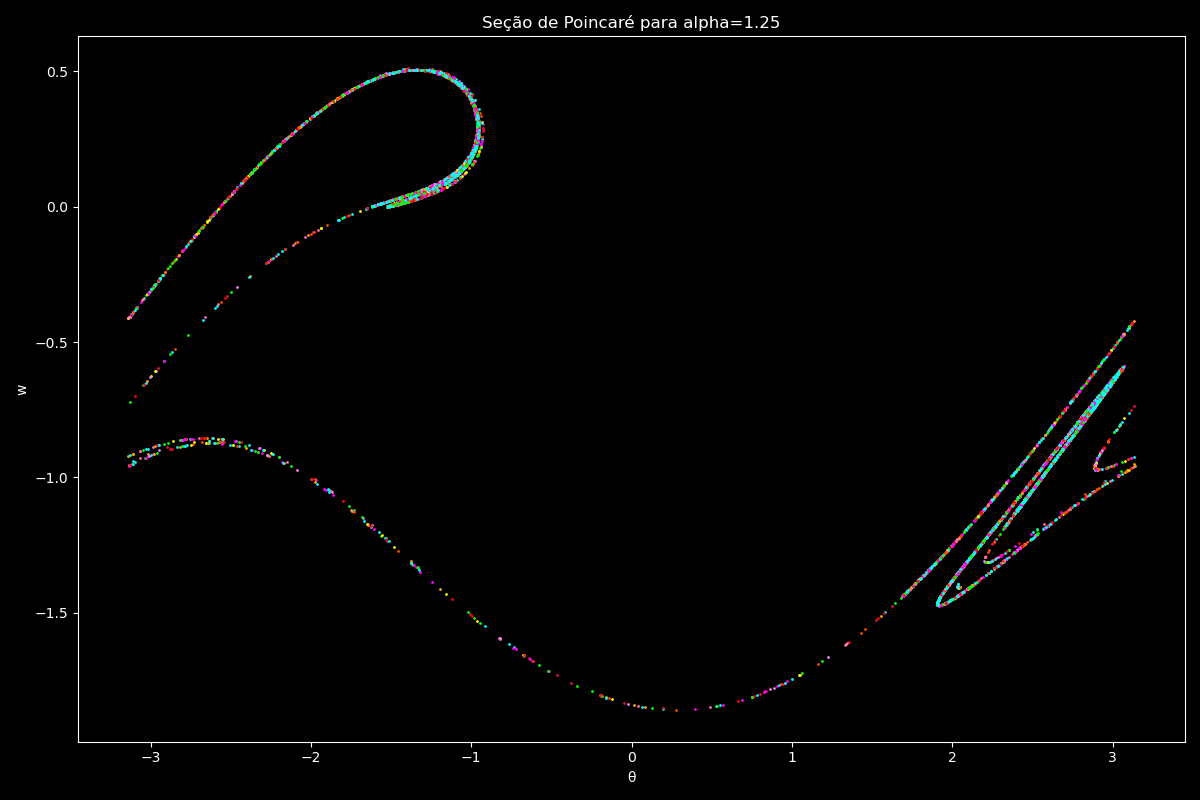
\includegraphics[width=\textwidth]{../tarefa-4c/secao_poincare_alpha_1.25.png}
\caption{Seção de poincaré para $\alpha = 1.25$.}
\end{figure}

\begin{figure}[H]
\centering
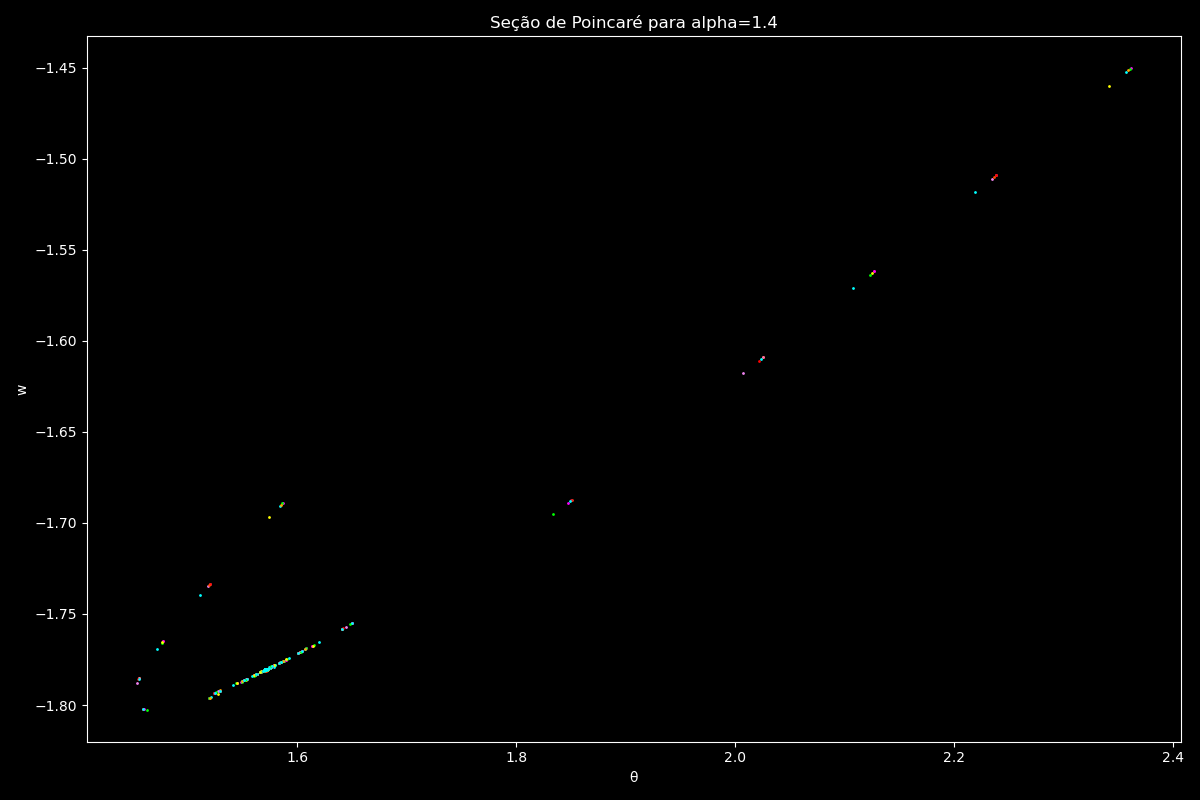
\includegraphics[width=\textwidth]{../tarefa-4c/secao_poincare_alpha_1.4.png}
\caption{Seção de poincaré para $\alpha = 1.4$.}
\end{figure}

\begin{figure}[H]
\centering
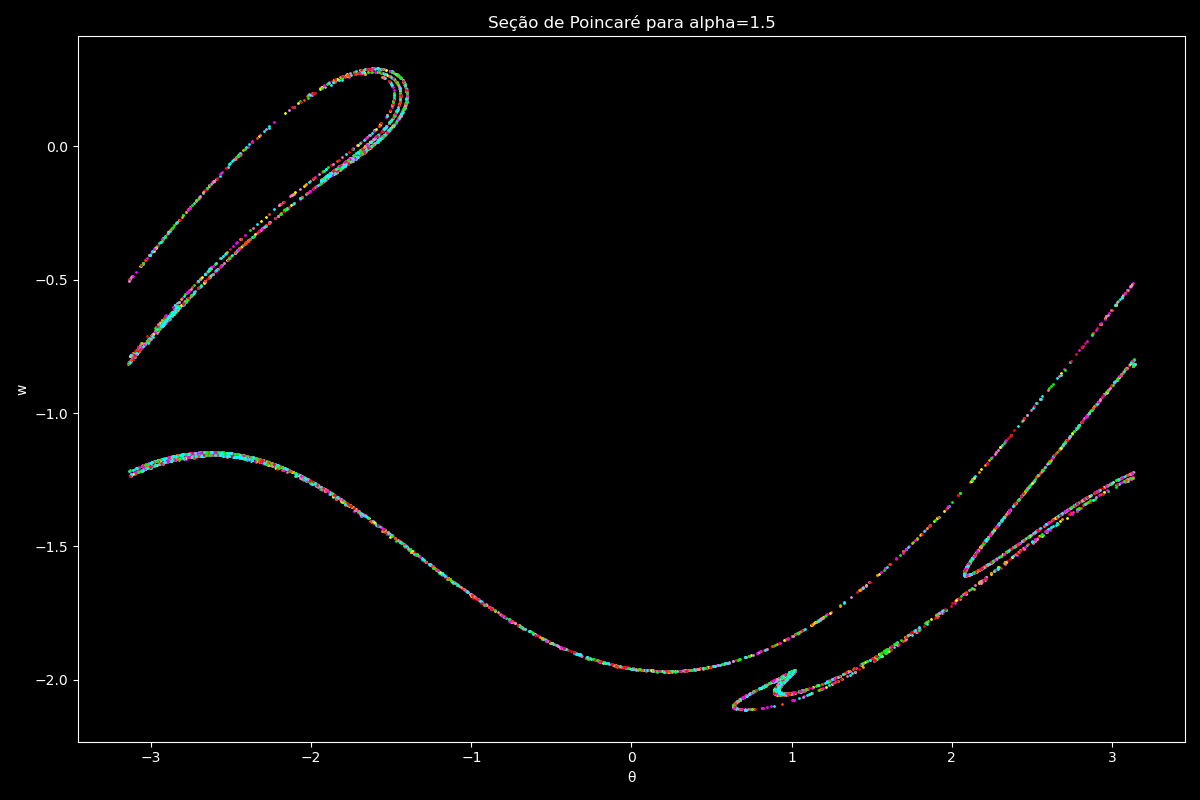
\includegraphics[width=\textwidth]{../tarefa-4c/secao_poincare_alpha_1.5.png}
\caption{Seção de poincaré para $\alpha = 1.5$.}
\end{figure}

Os gráficos são muito bonitos.

Podemos ver que para os osciladores periódicos, todos os pontos estão muito próximos ou até no mesmo ponto, enquanto que para os demais osciladores o gráfico é bem diferente. Vemos que mesmo com condições iniciais diferentes, os pontos vão se juntando para formar um padrão geométrico fractal. Muito lindo!

\subsection{d}

Aqui modificamos o programa da 4-a para calcular duas trajetórias e graficar $\delta_{\theta}$ e $\delta_{\omega}$. Segue o programa:

\begin{minted}[
	mathescape,
	linenos,
	fontsize=\footnotesize,
	framesep=2mm,
	breaklines]
	{fortranfixed}
      implicit real*8 (a-h, o-z)

      pi = 4.d0*datan2(1.d0,1.d0)

      w0 = 0d0
      teta0 = 0d0!pi*30d0/180d0
      teta0original = teta0
      total_tau = 5d0*2d0*pi

      write(*,*)"insira o total tau"
      read(*,*)total_tau

      dtau = 1d-3
      iteracoes = int(total_tau/dtau)

      gamma = 0.5d0
      ani = (2d0)/(3d0)

      tetanovo = 0d0
      wnovo = 0d0
      tetanewnovo = 0d0
      wnewnovo = 0d0

      open(file='tarefa-4d-teta.dat', unit=1)
      open(file='tarefa-4d-w.dat', unit=2)

      write(*,*)"Insira alpha"
      read(*,*)alpha

      write(*,*)"Insira t_trans"
      read(*,*)t_trans

      !write(*,*)"Insira teta0new"
      !read(*,*)teta0new
      write(*,*)"Insira w0new"
      read(*,*)w0new

      teta0new=0d0

      dteta = 0d0
      dw = 0d0

      do i=1,iteracoes
         tempo = dble(i)*dtau

         dteta = abs(teta0 - teta0new)
         dw = abs(w0 - w0new)


         if (tempo.gt.t_trans) then
            write(1,*) tempo, dteta
            write(2,*) tempo, dw
        endif

         wnovo = w0 -
     &   (dsin(teta0) + gamma*w0 - alpha*dsin(ani*tempo))*dtau

         wnewnovo = w0new -
     &   (dsin(teta0new) + gamma*w0new - alpha*dsin(ani*tempo))*dtau

         tetanovo = teta0 + wnovo*dtau
         tetanewnovo = teta0new + wnewnovo*dtau

         w0 = wnovo
         teta0 = tetanovo

         w0new = wnewnovo
         teta0new = tetanewnovo

         !teta0 = teta0 - dble(int(teta0/pi))*2d0*pi
         !teta0new = teta0new - dble(int(teta0new/pi))*2d0*pi
      end do

      end

\end{minted}

Para graficar e calcular o expoente de Lyapunov utilizamos o seguinte programa em Python:

\begin{minted}[
	mathescape,
	linenos,
	fontsize=\footnotesize,
	framesep=2mm,
	breaklines]
	{python}
import subprocess
import matplotlib.pyplot as plt
import numpy as np
import scipy.optimize as opt
from scipy.signal import find_peaks

# Configurar o estilo do gráfico
plt.style.use('ggplot')

# Parâmetros
alphas = [0.5, 0.75, 1.0, 1.25, 1.4, 1.5]
total_taus = [100, 100, 500, 50, 200, 200]
w0news = [1e-2, 1e-2, 1e-2, 1e-5, 1e-5, 1e-5]
t_trans = [20, 50, 30, 0, 0, 0]

# Compilar o código Fortran
subprocess.run(["gfortran", "-o", "tarefa-4d.exe", "tarefa-4d.f"])

def exponential_fit(x, lamb):
    return np.exp(lamb * x)

for total_tau, alpha, t_tran, w0new in zip(total_taus, alphas, t_trans, w0news):
    # Executar o programa Fortran com os valores atuais
    input_values = f"{total_tau:.8f}\n{alpha:.8f}\n{t_tran:.8f}\n{w0new:.8f}\n"
    subprocess.run(["./tarefa-4d.exe"], input=input_values.encode())

    # Ler os dados dos arquivos
    tempo, dteta = np.loadtxt('tarefa-4d-teta.dat', unpack=True)
    _, dw = np.loadtxt('tarefa-4d-w.dat', unpack=True)

    plt.figure(figsize=(10, 5))

    # Plotar dteta x tempo
    plt.subplot(211)
    plt.plot(tempo, dteta, label='Diferença em θ')

    # Plotar dw x tempo
    plt.subplot(212)
    plt.plot(tempo, dw, label='Diferença em ω')

    # Calcular e plotar a curva exponencial para os primeiros três alphas
    if alpha in alphas[:3] or alpha==1.5:
        # Encontrar picos/máximos locais
        peaks_dteta, _ = find_peaks(dteta)
        peaks_dw, _ = find_peaks(dw)

        # Ajustar a uma exponencial e plotar
        if len(peaks_dteta) > 1 and len(peaks_dw) > 1:
            popt_dteta, _ = opt.curve_fit(exponential_fit, tempo[peaks_dteta], dteta[peaks_dteta], p0=[0.1])
            popt_dw, _ = opt.curve_fit(exponential_fit, tempo[peaks_dw], dw[peaks_dw], p0=[0.1])

            lambda_teta = popt_dteta[0]
            lambda_w = popt_dw[0]

            plt.subplot(211)
            plt.plot(tempo, exponential_fit(tempo, lambda_teta), label=f'Fit Exponencial θ (λ={lambda_teta:.2f})')

            #if alpha != 1.5:
            plt.subplot(212)
            plt.plot(tempo, exponential_fit(tempo, lambda_w), label=f'Fit Exponencial ω (λ={lambda_w:.2f})')

    plt.subplot(211)
    plt.xlabel('Tempo')
    plt.ylabel('dteta')
    plt.legend()

    plt.subplot(212)
    plt.xlabel('Tempo')
    plt.ylabel('dw')
    plt.legend()

    plt.tight_layout()
    plt.savefig(f'diferencas_alpha_{alpha}.png')
    plt.close()

    # Imprimir os expoentes de Lyapunov calculados
    if alpha in alphas[:3]:
        print(f"Alpha: {alpha}, Lambda_theta: {lambda_teta:.2f}, Lambda_omega: {lambda_w:.2f}")

\end{minted}

Os gráficos são:

\begin{figure}[H]
\centering
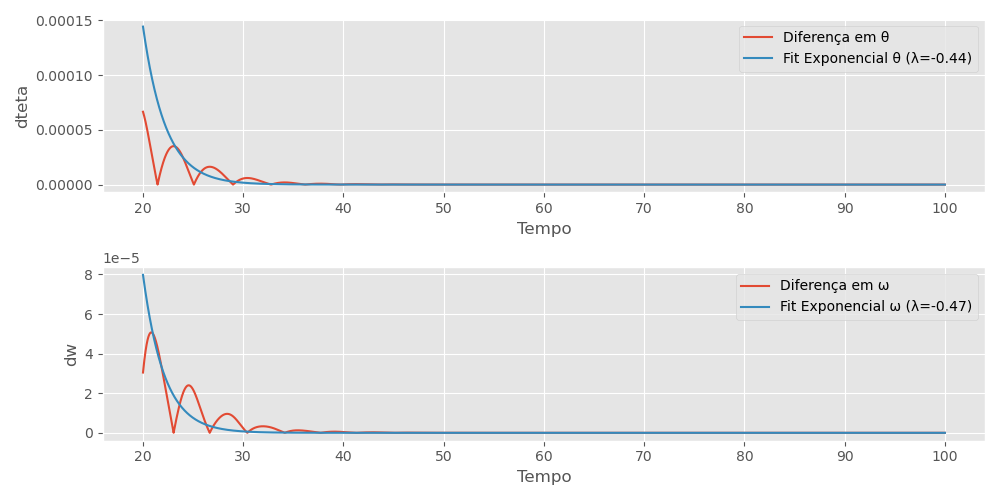
\includegraphics[width=\textwidth]{../tarefa-4d/diferencas_alpha_0.5.png}
\caption{Gráficos de $\delta_{\theta}$ e $\delta_{\omega}$ para $\alpha = 0.5$.}
\end{figure}

\begin{figure}[H]
\centering
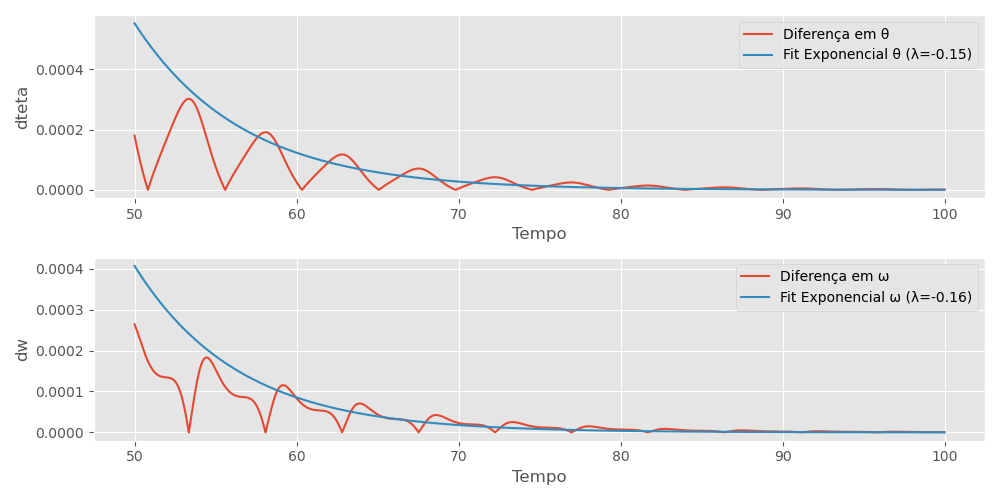
\includegraphics[width=\textwidth]{../tarefa-4d/diferencas_alpha_0.75.png}
\caption{Gráficos de $\delta_{\theta}$ e $\delta_{\omega}$ para $\alpha = 0.75$.}
\end{figure}

\begin{figure}[H]
\centering
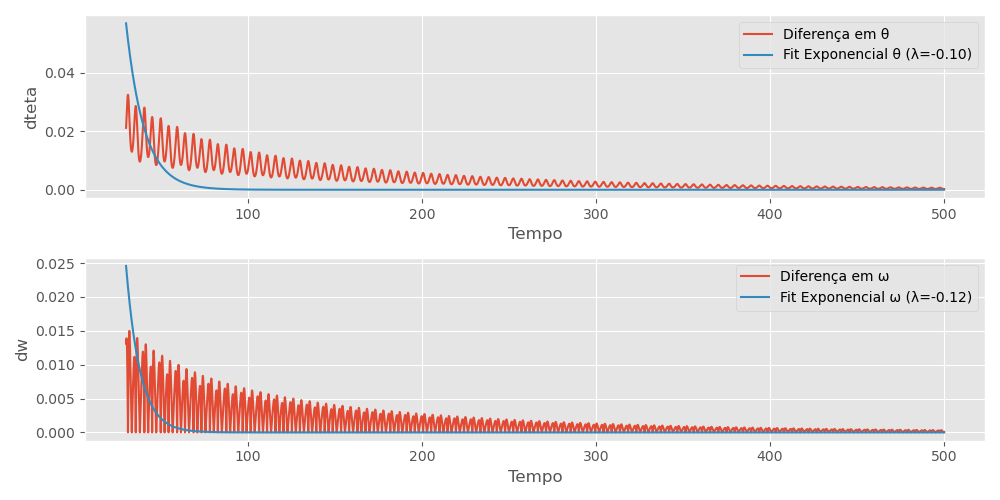
\includegraphics[width=\textwidth]{../tarefa-4d/diferencas_alpha_1.0.png}
\caption{Gráficos de $\delta_{\theta}$ e $\delta_{\omega}$ para $\alpha = 1.0$.}
\end{figure}

\begin{figure}[H]
\centering
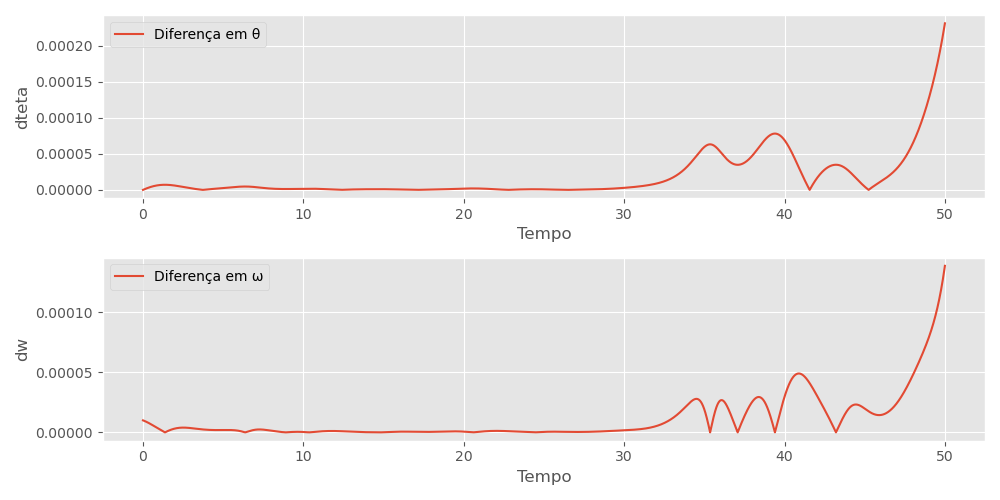
\includegraphics[width=\textwidth]{../tarefa-4d/diferencas_alpha_1.25.png}
\caption{Gráficos de $\delta_{\theta}$ e $\delta_{\omega}$ para $\alpha = 1.25$.}
\end{figure}

\begin{figure}[H]
\centering
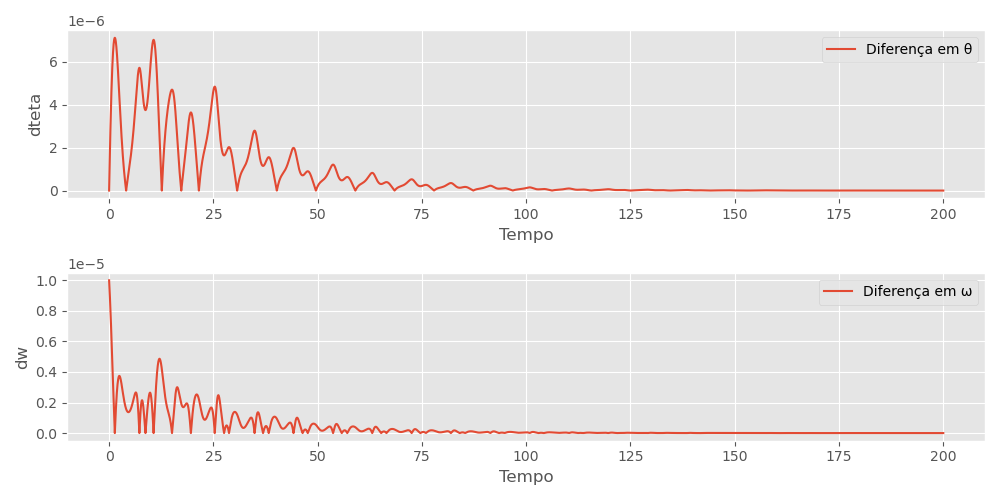
\includegraphics[width=\textwidth]{../tarefa-4d/diferencas_alpha_1.4.png}
\caption{Gráficos de $\delta_{\theta}$ e $\delta_{\omega}$ para $\alpha = 1.4$.}
\end{figure}

\begin{figure}[H]
\centering
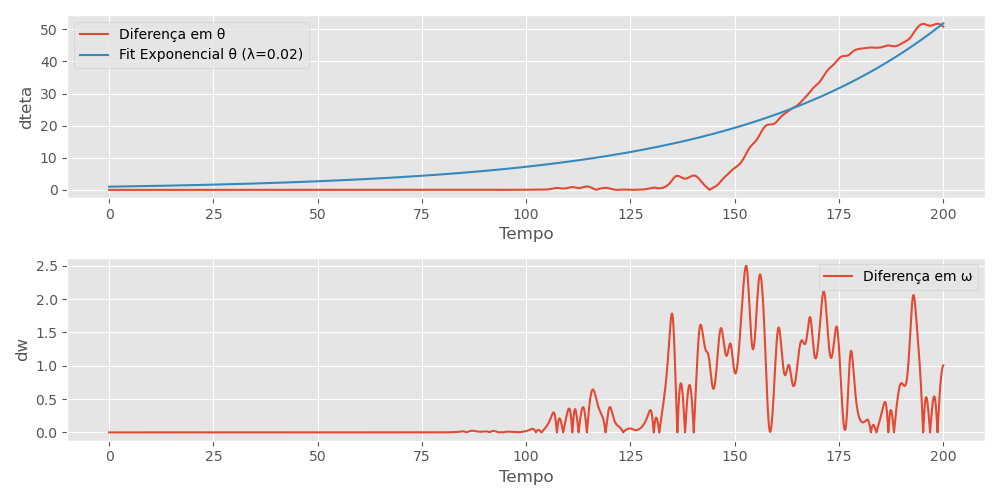
\includegraphics[width=\textwidth]{../tarefa-4d/diferencas_alpha_1.5.png}
\caption{Gráficos de $\delta_{\theta}$ e $\delta_{\omega}$ para $\alpha = 1.5$.}
\end{figure}

Nos casos periódicos, é possível ver uma curva exponencial decrescente e calcular assim o expoente. Vemos que os expoentes para $\theta$ e $\omega$ são aproximadamente equivalentes, mesmo que as curvas não sejam muito bem fitadas por eles. Enquanto que nos casos caóticos, as curvas não se assemelham muito a curvas exponenciais, não sendo possível fazer o fitting (pelo menos não o fitting automático do Python), exceto para o caso do $\theta$ de $\alpha = 1.5$. 

Não achamos necessário fazer tabela dos expoentes devido a eles serem facilmente visualizados nos gráficos. Acreditamos que a utilização do expoente de Lyapunov para os casos caóticos não é a mais adequada, ou há instruções faltando sobre como extraí-lo de forma correta, pois os gráficos claramente não são de forma exponencial.

\end{document}